\documentclass{article}

\usepackage{cmap} % чтобы работал поиск по PDF

\usepackage{caption}  %-  вставить в krctran перед описанием подписей caption (\renewcommand\@makecaption)
\usepackage{subcaption} % float figures side by side}  -  вставить в krctran перед описанием подписей caption (\renewcommand\@makecaption)
\usepackage{krctran}
\usepackage[utf8]{inputenc} % закомментировать в krctran.sty: \RequirePackage[cp1251]{inputenc}
\usepackage[pdftex]{graphicx} % закомментировать в krctran.sty
%\usepackage{caption}  %-  вставить в krctran перед описанием подписей caption (\renewcommand\@makecaption)
%\usepackage{subcaption} % float figures side by side}  -  вставить в krctran перед описанием подписей caption (\renewcommand\@makecaption)
\usepackage{textcomp}
\usepackage{xcolor}
\usepackage{algorithm2e}
\usepackage{float}
\usepackage{wrapfig}
%\usepackage[dvips]{graphicx}
\graphicspath{ {./pictures/} }

\begin{document}

\procname{Труды Карельского научного центра РАН\\ \No 0. 2015. С.~1--24}
\udk{УДК 81.32}

\rustitle{Обзор методов и алгоритмов разрешения \newline лексической многозначности: Введение}
\engtitle{Word-sense disambiguation methods and algorithms review: Introduction}

\rusauthor{Т.~В.~Каушинис$^2$,  А.~Н.~Кириллов$^1$,  Н.~И.~Коржицкий$^2$, А.~А.~Крижановский$^1$, А.~В.~Пилинович$^2$, И.~А.~Сихонина$^2$,  А.~М.~Спиркова$^2$, В.~Г.~Старкова$^1$, Т.~В.~Степкина$^2$, С.~С.~Ткач$^2$, Ю.~В.~Чиркова$^1$, А.~Л.~Чухарев$^1$,  Д.~С.~Шорец$^2$,  Д.~Ю.~Янкевич$^2$, Е.~А.~Ярышкина$^2$}
\engauthor{T.~V.~Kaushinis$^2$, A.~N.~Kirillov$^1$, N.~I.~Korzhitsky$^2$, A.~A.~Krizhanovsky$^1$, A.~V.~Pilinovich$^2$, I.~A.~Sikhonina$^2$, A.~M.~Spirkova$^2$, V.~G.~Starkova$^1$, T.~V.~Stepkina$^2$, S.~S.~Tkach$^2$, J.~V.~Chirkova$^1$, A.~L.~Chuharev$^1$, D.~S.~Shorets$^2$, D.~Y.~Yankevich$^2$, E.~A.~Yaryshkina$^2$}


\organization{$^1$Институт прикладных математических исследований Карельского научного центра РАН \\
$^2$Петрозаводский Государственный Университет}


\rusabstract{Разрешение лексической многозначности --- это задача выбора между разными значениями 
слов и словосочетаний в словаре в зависимости от контекста. 
В статье представлен краткий обзор методов и алгоритмов разрешения лексической многозначности. 



Представлены (1) методы, основанные на машинном обучении, 
(2) методы, не использующие никаких размеченных корпусов для различения значений слов, и 
(3) методы, использующие внешние словарные источники информации (машиночитаемые словари, тезаурусы, онтологии). 
Статья распространяется на правах свободной лицензии “CC Attribution”.
}
\engabstract{The word sense disambiguation (WSD) task is the classification task, where the goal is to predict the meaning of words and phrases with the help of surrounding text. The purpose of this short review is to acquaint the reader with the general directions of word sense disambiguation methods and algorithms. The paper consists of three main parts: (1) supervised (machine learning) approaches to WSD, (2) unsupervised approaches based on unlabeled corpora and (3) knowledge-based approaches to WSD, where machine-readable dictionaries, thesauri, ontologies are used. This work is licensed under the CC Attribution license.}

\ruskeywords{алгоритм, метод, разрешение лексической многозначности.}
\engkeywords{algorithm, method, word-sense disambiguation.}

\maketitle

\begin{articletext}

\section{Введение}
В статье представлен обзор методов и алгоритмов разрешения лексической многозначности (word-sense disambiguation или WSD). Верный выбор в словаре одного из значений многозначного слова или фразы в зависимости от контекста и является успешным результатом решения WSD-задачи.

Приведем несколько примеров употребления слова <<коса>> и <<косой>>, найденных с помощью Национального корпуса русского языка (http://ruscorpora.ru) по запросу <<коса>>:

\begin{enumerate}
\item Поп сам в первой \textit{\underline{косе}} идет, но прихожане не торопятся, смотрят на солнышко и часа через полтора уже намекают, что обедать пора. {\footnotesize[\textit{М. Е. Салтыков-Щедрин. Мелочи жизни (1886-1887)}]}
\item Но работа даже и после этого идет все вялее и вялее; некоторые и \textit{\underline{косы}} побросали. {\footnotesize[\textit{М. Е. Салтыков-Щедрин. Мелочи жизни (1886-1887)}]}
\item В особенности жестоко было крепостное право относительно дворовых людей: даже волосы крепостных девок эксплуатировали, продавая их \textit{\underline{косы}} парикмахерам. {\footnotesize[\textit{М. Е. Салтыков-Щедрин. Мелочи жизни (1886-1887)}]}
\item Это одинокая скала, соединяющаяся с материком намывной \textit{\underline{косой}} из песка и гальки. {\footnotesize[\textit{В. К. Арсеньев, «По Уссурийскому краю», 1917 г.}]}
\item Первая черепашка подскочила к гвардейцу и воткнула ему в спину сверкающий \textit{\underline{косой}} меч. {\footnotesize[\textit{Виктор Пелевин. S.N.U.F.F, 2011}]}
\end{enumerate}

Первые четыре примера дают три разных значения существительного <<коса>>: ряд косарей, сельскохозяйственное орудие, заплетенные волосы, протяженная речная отмель. Последний пример содержит прилагательное <<косой>>, совпадающее с одной из форм существительного <<коса>>. Все эти значения и часть речи читатель легко определяет по контексту. 

Именно многозначность слов, их неоднозначность и зависимость значений слов от контекста являются причиной возникновения такой задачи и одновременно обуславливают сложность ее решения. Уверенное решение WSD-задачи необходимо во многих приложениях, связанных с автоматической обработкой текста (информационный поиск, машинный перевод и т.п.) и, на наш взгляд, является предтечей искусственного интеллекта.

Для этой задачи известно большое количество алгоритмов и методов решения, которые можно разделить на \cite{Lukash 2011}, \cite{Navigli 2009}: 

\begin{itemize}
\item WSD-методы с учителем (\textit{supervised}) --- методы, базирующиеся на машинном обучении и работающие на размеченных корпусах текстов; 
\item WSD-методы без учителя (\textit{unsupervised}), не использующие никаких размеченных корпусов для различения значений слов.
\end{itemize}

Другая классификация методов строится на противопоставлении используемых ресурсов \cite{Navigli 2009}:
\begin{itemize}
\item WSD-методы, основанные на знаниях (\textit{knowledge-based}); в этих методах используются внешние словарные источники информации (машиночитаемые словари, тезаурусы, онтологии);
\item WSD-методы, основанные на корпусах текстов (\textit{corpus-based}).
\end{itemize}

Также применяются комбинации этих методов.

На сегодняшний день на русском языке нет, по-видимому, достаточно объёмных и серьёзных обзоров по разрешению многозначности. Наиболее полное описание истории развития методов (20 страниц) есть в диссертации Д. Ю. Турдакова \cite{Trudakov 2010}. Такое положение дел послужило одной из причин написания этой статьи, которая послужит заделом для полновесного обзора по данной теме.

Далее будут представлены примеры методов и алгоритмов разрешения лексической многозначности, разбитые на три группы: 
\begin{itemize}
\itemс использованием машинного обучения: метод ансамбля байесовских классификаторов, нейронные сети, бустинг как метод улучшения точности алгоритма обучения, сравнение методов машинного обучения;
\itemбез машинного обучения: различение значений на основе контекстных векторов, расширенных словарными значениями; поиск и кластеризация похожих слов; кластеризация фрагментов биомедицинских текстов; кластеризация посредством комитетом;
\itemметоды, основанные на знаниях: лексические цепочки, сочетаемостные ограничения на основе байесовских сетей.
\end{itemize}
 Данная статья является <<введением>> в проблематику WSD, поскольку эта тема является чрезвычайно обширной и существуют сотни интересных работ по каждому из указанных направлений.

\bfullwidth
\begin{center}
\section{WSD-методы с учителем}
\end{center}
\efullwidth

\section{Разрешение лексической многозначности методом ансамбля байесовских классификаторов}

\begin{flushright}
\textit{А. Л. Чухарев, Т. В. Каушинис}
\end{flushright}

В работе Педерсена \cite{Pedersen 2000} рассматривается подход к разрешению лексической многозначности слов (WSD), подразумевающий создание ансамбля наивных байесовских классификаторов, каждый из которых основан на оценке вероятности вхождения определенных слов в контекст целевого слова, значение которого определяется.
\parindent=0,5cm

При разрешении лексической многозначности, представленной как задача обучения с учителем, применяют статистические методы и методы машинного обучения к размеченному корпусу. В таких методах словам корпуса, для которых указано значение, соответствует набор языковых свойств. Педерсен \cite{Pedersen 2000} относит к языковым свойствам два вида особенностей: так называемые простые лексические особенности (shallow lexical features) и более сложные лингвистически обусловленные особенности (lingvistically motivated features). К первым относятся совместная встречаемость слов (co-occurence) и словосочетания (collocations), в то время как вторые включают в себя такие свойства как часть речи и отношение действие-объект. Обычно алгоритмы обучения строят модели классификаторов значений по этим языковым свойствам.

Автор статьи \cite{Pedersen 2000} предлагает подход, основанный на объединении ряда простых классификаторов в ансамбль, который разрешает многозначность с помощью голосования простым большинством голосов. Педерсен утверждает \cite{Pedersen 2000}, что, во-первых, более сложные алгоритмы обычно не улучшают точность разрешения. Во-вторых, совместная встречаемость слов и словосочетаний имеют большее влияние на точность разрешения, чем оперирование более сложной лингвистической информацией.
\parindent=0,5cm


В рассматриваемой статье \cite{Pedersen 2000} в ансамбль объединяются наивные байесовские классификаторы. При таком подходе предполагается, что все переменные, участвующие в представлении проблемы, --- условно независимы при фиксированном значении переменной классификации. В проблеме разрешения лексической многозначности существует понятие контекста, в котором встречается многозначное слово. Этот контекст представляется в виде функции переменных $(F_1, F_2, \ldots , F_n)$, а значение многозначного слова представлено в виде классификационной переменной (S). Все переменные бинарные. Переменная, соответствующая слову из контекста, принимает значение ИСТИНА, если это слово находится на расстоянии определенного количества слов слева или справа от целевого слова. Совместная вероятность наблюдения определенной комбинации переменных контекста с конкретным значением слова выражается следующим образом: 
\\
\\
$p(F_1, F_2, \ldots , F_nS) = p(S)\Pi^n_{i=1}p(F_i \vee S)$ 
\\
\\
где $p(S)$ и $p(F_i|S)$ --- параметры данной модели. Для оценки параметров достаточно знать частоты событий, описываемых взаимозависимыми переменными $(F_i,S)$. Эти значения соответствуют числу предложений, где слово, представляемое $F_i$, встречается в некотором контексте многозначного слова, упомянутого в значении $S$. Если возникают нулевые значения параметров, то они сглаживаются путем присвоения им по умолчанию очень маленького значения. После оценки всех параметров модель считается  обученной и может быть использована в качестве классификатора.
\parindent=0,5cm

Контекст в \cite{Pedersen 2000} представлен в виде bag-of-words (модель «мешка слов»). В этой модели выполняется следующая предобработка текста: удаляются знаки препинания, все слова переводятся в нижний регистр, все слова приводятся к их начальной форме (лемматизация). 
В \cite{Pedersen 2000} контексты делятся на два окна: левое и правое. В первое попадают слова, встречающиеся слева от неоднозначного слова, и, соответственно, во второе --- встречающиеся справа.
\parindent=0,5cm

Окна контекстов могут принимать 9 различных размеров: 0, 1, 2, 3, 4, 5, 10, 25 и 50 слов. Первым шагом в ансамблевом подходе является обучение отдельных наивных байесовских классификаторов для каждого из 81 возможных сочетаний левого и правого размеров окон. В статье  \cite{Pedersen 2000} наивный байесовский классификатор $(l,r)$ включает в себя $l$ слов слева от неоднозначного слова и $r$ слов справа. Исключением является классификатор (0,0), который не включает в себя слов ни слева, ни справа. В случае нулевого контекста классификатору присваивается \textbf{априорная вероятность} многозначного слова (равная  вероятности  встретить наиболее употребимое значение).
\parindent=0,5cm

Следующий шаг в \cite{Pedersen 2000} при построении ансамбля --- это выбор классификаторов, которые станут членами ансамбля. 81 классификатор группируется в три общие категории, по размеру окна контекста. Используются три таких диапазона: узкий (окна шириной в 0, 1 и 2 слова), средний (3, 4, 5 слов), широкий (10, 25, 50 слов). Всего есть 9 возможных комбинаций, поскольку левое и правое окна отделены друг от друга. Например, наивный байес (1,3) относится к диапазону категории (узкий, средний) поскольку он основан на окне из одного слова слева и окне из трех слов справа.  Наиболее точный классификатор в каждой из 9 категорий диапазонов выбирается для включения в ансамбль. Затем каждый из 9 членов классификаторов голосует за наиболее вероятное значение слова с учетом контекста. После этого ансамбль разрешает многозначность путем присвоения целевому слову значения, получившего наибольшее число голосов. 
\parindent=0,5cm

\textbf{Экспериментальные данные.} Для экспериментов были выбраны английские слова \textit{line} и \textit{interest.} Источником статистических данных по этим словам послужили работы \cite{Leacock 1993}, \cite{Bruce 1994}. В статье приводится информация о частоте использования шести значений для каждого из этих слов (Табл.~\ref{tbl3}, Табл.~\ref{tbl4}). 

\begin{table}[H]
\centering
\caption{Число употреблений слова \textit{line} (столбец \textit{count}) для шести наиболее часто встречаемых значений (значения из те\-за\-уру\-са WordNet, столбец \textit{sense}) по данным корпусов \textit{ACL/DCI Wall Street Journal и American Printing House for the Blind}}
\begin{tabular}{|c|c|}
\hline
sense & count\\
\hline
product & 2218\\
written or spoken text & 405\\
telephone connection & 429\\
formation of people or things; queue & 349\\
an artificial division; boundary & 376\\
a thin, flexible object; cord & 371\\
\hline
total & 4148\\
\hline
\end{tabular}
\label{tbl3}
\end{table}

\begin{table}[H]
\centering
\caption{Число употреблений слова \textit{interest} (столбец \textit{count}) для шести наиболее часто встречаемых значений (значения из словаря Longman Dictionary of Contemporary English, столбец \textit{sense}). Этот набор данных был получен в 1994 году Брюсом и Виебе \cite{Bruce 1994} путем указания значений для всех вхождений слова \textit{interest} в корпус ACL/DCI Wall Street Journal}
\begin{tabular}{|c|c|}
\hline
sense & count\\
\hline
money paid for the use of money & 1252\\
a share in a company or business & 500\\
readiness to give attention & 361\\
advantage, advancement or favor & 178\\
activity that one gives attention to & 66\\
causing attention to be given to & 11\\
\hline
total & 2368\\
\hline
\end{tabular}
\label{tbl4}
\end{table}


\parindent=0,5cm
\textbf{Результаты экспериментов.} Итогом проделанной работы стали обучение и проверка 81 наивного байесовского классификатора на многозначных словах \textit{line} и \textit{interest.} Точность разрешения лексической многозначности составила 89\% для слова \textit{interest} и 88\% для слова \textit{line.} В \cite{Pedersen 2000} было получено, что ансамбль классификаторов с голосованием простым большинством дает более высокую точность, чем взвешенное голосование. Например, для слова \textit{interest} при голосовании простым большинством точность составила 89\%, а взвешенное голосование дало только 83\%.



\bfullwidth
\section{WSD на основе нейронных сетей, построенных по данным машиночитаемых словарей}
\efullwidth

\begin{flushright}
\textit{А. Н. Кириллов}
\end{flushright}

\parindent=0,5cm

Использование нейронных сетей (NN)  для WSD было предложено в 80-е гг. в работах \cite{COTTRELL 1983,WALTZ 1985}. В типичной NN на вход   подается   слово, значение которого требуется установить, т.е. целевое (\textit{target}) слово, а также --- контекст (фраза) его содержащий. Узлы выхода соответствуют различным значениям слова. В процессе обучения, когда значение тренировочного целевого слова известно, веса связующих узлы соединений (связей), настраиваются таким образом, чтобы по окончании обучения выходной узел, соответствующий истинному значению целевого слова, имел наибольшую активность. Веса соединений могут быть  положительными или отрицательными, и настраиваются посредством рекуррентных алгоритмов (алгоритм обратного распространения ошибки,  рекуррентный метод наименьших квадратов и т.д.). Сеть может содержать скрытые (hidden) слои, состоящие из узлов, соединенных как прямыми, так и обратными связями. Для представления входной информации обычно используется одна из двух схем:  распределенная (distributed) или локалистская (localist ) (\cite{Hinton 1986}, \cite{COTTRELL 1989}, \cite{Azzini}). 

В работе \cite{VERONIS 1990} описан метод автоматического построения \textbf{\textit{очень больших нейронных сетей}} (VLNN) с помощью текстов, извлекаемых из машиночитаемых словарей (MRD), и рассмотрено использование этих сетей в задачах разрешения лексической неоднозначности. Поясним основную идею VLNN.  Широко известен метод Леска \cite{LESK 1986}  использования  информации  из MRD для  задачи  WSD.  Суть этого метода состоит в вычислении  так называемой \textit{степени пересечения}, т.е.  количества общих слов в словарных определениях слов из контекста (<<окна>>) условного размера, содержащего целевое слово. Основной недостаток метода Леска --- зависимость  от  словарной  статьи, то есть от слов, входящих в нее. Стратегия преодоления  этого  недостатка --- использование словарных статей, определяющих слова, входящие в другие словарные статьи, начиная со словарных статей, соответствующих  словам  из  контекста. Таким образом, образуются  достаточно  длинные   пути  из слов, входящих в словарные статьи. Эта  идея  лежит  в  основе  топологии VgN. В работе \cite{VERONIS 1990}  для построения  VLNN использован  словарь  Collins  English  Dictionary.

\textbf{Топология сети.} Целевое слово представлено  узлом, соединенным активирующими  связями со смысловыми узлами, представляющими все возможные значения слова, имеющиеся  в словарных статьях. Каждый смысловой узел, в свою очередь, соединен  активирующими  связями с узлами, представляющими  слова в словарной статье, соответствующей толкованию данного значения. Процесс соединения повторяется многократно, создавая сверхбольшую сеть взаимосвязанных узлов. В идеале сеть может содержать весь словарь. Авторы, по практическим соображениям, ограничиваются несколькими тысячами узлов и 10–20 тысячами соединений. Слова представлены своими леммами (каноническими формами). Узлы, представляющие различные значения данного слова, соединены запрещающими (inhibitory) связями.  

\textbf{Алгоритм.} При запуске сети первыми активируются узлы входного  слова  (согласно принятой кодировке). Затем  каждый  входной узел посылает активирующий сигнал своим смысловым узлам, с которыми он соединен. В результате  сигналы распространяются по всей сети в течение определенного числа циклов. В каждом цикле узлы слова и  его значений получают обратные сигналы от узлов, соединенных с ними. Узлы конкурирующих значений посылают взаимно подавляющие сигналы.  Взаимодействие  сигналов  обратной  связи  и  подавления,  в соответствии со стратегией <<победитель получает все>>, позволяет увеличить активацию узлов-слов и соответствующих им правильных узлов-значений,  одновременно  уменьшая  активацию  узлов,  соответствующих неправильным значениям. После нескольких десятков  циклов сеть стабилизируется  в  состоянии, в котором активированы  только узлы-значения с наиболее активированными связями  с    узлами-словами. При обучении сети  используется  метод  обратного  распространения (\textit{back  propagation}).

\section{Краткое введение в бустинг}

\begin{flushright}
\textit{Т. Степкина, Ю. В. Чиркова}
\end{flushright} 

В статье \cite{Freund 1999} говорится о бустинге --- общем методе улучшения точности алгоритма обучения. В работе приводится алгоритм AdaBoost с описанием необходимой теории бустинга, а также показывается связь с методом опорных векторов и объясняются причины, по которым переобучение не влияет на бустинг.  

Бустинг --- это общий и доказуемо-эффективный метод получения очень точного правила предсказания путем комбинирования грубых и умеренно неточных эмпирических правил \cite{Freund 1999}. Метод бустинга разработан на основе модели обучения "PAC" (probably approximately correct learning).

Алгоритм AdaBoost был предложен в 1995 году Фройндом и Шапиро \cite{Freund 1996}. В нём исправлены многие недостатки предыдущих алгоритмов бустинга.

AdaBoost является адаптивным алгоритмом \cite{Freund 1999}, поскольку он может адаптироваться к уровням ошибок отдельных слабых гипотез. В названии "Ada" является сокращением от «adaptive» (адаптивный).

На вход алгоритма поступает обучающая выборка $(x_i;y_i);..;(x_m;y_m)$, где каждый элемент $x_i$ принадлежит некоторому домену или признаковому пространству $X$, и каждая метка $y_i$ принадлежит некоторому набору меток $Y$. Для каждого обучающего примера $i$ вес распределения для целых $t$ обозначается $D_t$ $(i)$, где $t$ --- это шаг алгоритма. За начальное распределение весов принимается $D_1$ $(i)= 1/m$. Пусть метки принимают значения из множества  $Y=\{-1,1\}$. 

Далее на каждом шаге $t$, где $t = 1 \ldots T$, выполняется обучение слабого обучаемого с использованием текущего распределения $D_t$, после чего строится слабая гипотеза $h_t: X \to \{-1; 1\}$ с ошибкой первого рода $\epsilon_t=\Sigma_{\displaystyle (i:h_t (x_i)\ne y_i)}D_t(i)$, по которой выбирается уровень значимости $\alpha_t=\frac{1}{2}ln(\frac{\displaystyle 1-\epsilon_t}{\displaystyle \epsilon_t})$ и строится новое распределение для следующего шага
%\bfullwidth
%\begin{equation*}
$$
D_{t+1}(i)=\frac{D_{t^i}}{Z_t} \times 
\begin{cases}
e^{-\alpha t}\text{, если }h_t (x_i) = y_i \\
e^{\alpha t}\text{, если }h_t (x_i)\ne y_i
\end{cases}
=
$$
$$
= \frac{D_t (i)exp(-\alpha_t y_i h_t (x_i))}{Z_t}. 
$$
%\end{equation*}
%\efullwidth

Конечная гипотеза $H(x)$ ---  это среднее из большинства решений $T$ слабых гипотез, где $\alpha_t$ --- вес, присвоенный гипотезе $h_t$.

%\bfullwidth
%\begin{equation*}
$$
H(x)=sign(\sum_{t=1}^T\alpha_t h_t(x))
$$
%\end{equation*}
%\efullwidth

Идея алгоритма заключается в выборе набора весов для обучающей выборки. Первоначально все веса примеров устанавливаются одинаково, но на каждом круге цикла веса неправильно классифицированных по гипотезе $h_t$ примеров увеличиваются, таким образом, получают веса, которые относятся к сложным примерам.

Основное теоретическое свойство AdaBoost --- это способность алгоритма уменьшать ошибку обучения \cite{Freund 1999}. Фройнд и Шапиро показали, что, так как каждая слабая гипотеза немного лучше случайного выбора, ошибка обучения уменьшается с экспоненциальной скоростью.

В статье \cite{Freund 1999} показано как ограничена ошибка обобщения конечной гипотезы в терминах ошибки обучения, размера выборки m, VC размерности (размерности Вапника --- Червоненкиса \cite{Schapire 1997}) пространства слабых гипотез и количества циклов Т. Также получена граница, не зависящая от Т. Это показывает, что бустинг AdaBoost не подвержен эффекту переобучения.

Так как ошибка обучения и ошибка обобщения ограничены, как показано в статье \cite{Freund 1999}, этот алгоритм действительно является бустинговым алгоритмом в том смысле, что он может эффективно преобразовать слабый алгоритм обучения в сильный, который может породить гипотезу со сколь угодно малой частотой ошибок, имея достаточное количество данных.

После того, как авторы рассмотрели бинарный случай, где целью является различие лишь между двумя возможными классами, они переходят к рассмотрению мультиклассного, более приближенного к реальности. Есть несколько способов приведения AdaBoost к мультиклассному случаю. Самое простое обобщение называется AdaBoost.M1 \cite{Freund 1997}, которое является приемлемым, если слабый обучаемый может достичь достаточно высокой точности на распределениях, созданных AdaBoost. Тем не менее, этот метод завершается неудачно, если слабый ученик не может достичь хотя бы 50\% точности при работе на этих  распределениях. Для такого случая было разработано несколько методов:

\begin{enumerate}
\item Методы, которые работают за счет преобразования мультиклассной задачи в большую бинарную задачу или в набор бинарных задач. Однако, эти методы требуют дополнительных усилий в разработке слабого алгоритма обучения.
\item Технология, которая включает в себя метод Диттерича и Бакири --- метод выходных кодов, исправляющих ошибки \cite{Schapire 1997}.
\end{enumerate}

AdaBoost обладает определенными преимуществами. Его быстро и просто запрограммировать. Он не имеет никаких параметров для настройки, за исключением количества циклов. Он не требует никаких предварительных знаний о слабом обучаемом и поэтому может быть скомбинирован с любым методом для нахождения слабых гипотез.

Недостатки метода заключаются в следующем. Фактическая производительность бустинга на конкретной задаче явно зависит от данных и слабого обучаемого. Теоретически, бустинг может выполниться плохо, если данных недостаточно, слабые гипотезы слишком сложные, или наоборот слишком слабые. Также бустинг особенно восприимчив к шуму.

AdaBoost был протестирован эмпирическим путем многими исследователями. Например, Фройнд и Шапиро проверили AdaBoost на множестве эталонных наборов данных UCI \cite{Merz 1998} с использованием C4.5 \cite{Quinlan 1993} как слабого алгоритма обучения, а также алгоритм, который находит самое лучшее дерево решений с одним тестом. После проведения эксперимента был сделан вывод, что бустинг даже слабых деревьев решений с одним тестом, как правило, дает хорошие результаты, в то время как бустинг C4.5, как правило, дает алгоритм дерева принятия решений значительно улучшенной производительности.

Почти во всех этих экспериментах и для всех показателей эффективности бустинг работает так же хорошо или значительно лучше, чем в других методах испытаний. Бустинг также применяется к фильтрации текстов, проблемам ранжирования и проблемам классификации, возникающих при обработке естественного языка.

\section{Сравнительные эксперименты в WSD: роль предпочтений в машинном обучении}

\begin{flushright}
\textit{Н. И. Коржицкий}
\end{flushright}

В заключение главы, посвященной разрешению многозначности, приведем эксперементальное сравнение методов. В работе Рэймонда Муни \cite{Mooney 1996} представлено одно из первых сравнений разных по природе методов WSD на одних и тех же данных. В статье \cite{Mooney 1996} проведена серия экспериментов, в которых сравнивалась способность различных обучающихся алгоритмов определять значение слова в зависимости от контекста. 

В машинном обучении под термином \textit{bias} (пристрастие, тенденция, предпочтение)  понимается любое основание для выбора одного обобщения другому, вместо строгого соответствия примерам \cite{Mooney 1996}. В деревьях принятия решений предпочтение (\textit{bias}) отдается простым деревьям решений, в нейронных сетях --- линейным пороговым функциям, а в байесовском классификаторе --- функциям, учитывающим условную независимость свойств. Чем лучше <<предпочтение>> обучающегося алгоритма соответствует характеристикам конкретной задачи, тем лучше будет результат. Большинство обучающихся алгоритмов обладают <<предпочтением>> наподобие Бритвы Оккама, в таких алгоритмах выбираются гипотезы, которые могут быть представлены меньшим количеством информации на каком-нибудь языке представлений. Однако компактность, с которой (деревья решений, дизъюнктивная нормальная форма, сети с линейным пороговым значением) представляют конкретные функции --- может существенно различаться. Поэтому различные <<предпочтительные>> оценки могут работать лучше или хуже в конкретных задачах. Одной из основных целей в машинном обучении является поиск <<предпочтений>> с целью решения прикладных практических задач.
\parindent=0,5cm

Выбор правильного <<предпочтения>> и обучающегося алгоритма является сложной задачей. Простым подходом является автоматизация выбора метода при помощи внутренней перекрестной валидации. Другой подход meta-learning заключается в том, чтобы обучиться набору правил (или другому классификатору), предсказывающему, когда обучающийся алгоритм будет срабатывать наилучшим образом на примере с набором свойств присущих проблеме.
\parindent=0,5cm

Описанный в \cite{Mooney 1996} эксперимент заключается в определении значения слова \textit{line} (англ. \textit{линия}) среди 6 возможных вариантов (\textit{строка, ряд, дивизия, телефон, веревка, продуктовая линия}). Данные для проведения экспериментов взяты из работы \cite{Leacock 1993}.  

Для получения обучающей выборки брались предложения со словом \textit{line}, и им в соответствие ставилось одно из 6 значений. Распределение значений неравномерно: включение в список иточников журнала The Wall Street Journal привело к тому, что одно из значений встречалось в 5 раз чаще всех остальных \cite{Leacock 1993}.
\parindent=0,5cm

\bfullwidth
\begin{table}[H]
\centering
\caption{Шесть значений слова \textit{line} из Английского Викисловаря и Русского Викисловаря}
\begin{tabular}{|m{2cm}|m{2cm}|m{6cm}|m{4cm}|}

\hline
\textbf{ключевое слово} & \textbf{перевод} & \textbf{толкование на английском (Английский Викисловарь)} & \textbf{толкование на русском (Русский Викисловарь)}\\
\hline
text & строка & A small amount of text & ряд слов, букв или иных знаков, написанных или напечатанных в одну линию \\
\hline
formation & ряд & A more-or-less straight sequence of people, objects, etc., either arranged as a queue or column and often waiting to be processed or dealt with, or arranged abreast of one another in a row (and contrasted with a column), as in a military formation & несколько объектов, расположенных в линию или следующих один за другим\\
\hline
division & дивизия & A formation, usually made up of two or three brigades & тактическое воинское соединение \\
\hline
phone & телефон & The wire connecting one telegraphic station with another, a telephone or internet cable between two points: a telephone or network connection & то же, что телефонный номер \\
\hline
cord & веревка & A rope, cord, string, or thread, of any thickness  & гибкое и длинное изделие, — чаще всего сплетенное или свитое из льняных (или пеньковых, полимерных и т. п.) волокон или прядей \\
\hline
product & продуктовая линия & The products or services sold by a business, or by extension, the business itself & совокупность однородной продукции единого назначения  \\
\hline
\end{tabular}
\label{tbl5}
\end{table}
\efullwidth

\parindent=0,5cm

В работе \cite{Charles 1993} было установлено, что наиболее эффективными при решении задачи WSD являются алгоритмы на основе дерева решений (decision tree). Данный класс методов обходил по точности и скорости работы класс нейронных сетей. Другие исследования \cite{Mooney 1995} показали, что класс методов индуктивного логического программирования (inductive logic programming) справляется с задачей разрешения лексической многозначности слова лучше алгоритмов на основе дерева решений. 
\parindent=0,5cm

В серии экспериментов в \cite{Mooney 1996} сравнивались следующие методы: байесовский классификатор, перцептрон, C4.5, метод k-ближайших соседей и модификации алгоритма FOIL: PFOIL-DLIST, PROIL-DNF, PFOIL-CNF. Все алгоритмы были реализованы на языке Common Lisp, за исключением C4.5, который был написан на языке C.
\parindent=0,5cm

После проведения сравнительных экспериментов, заключавшихся в обучении и определении значения слова \textit{line,} было выяснено, что байесовский классификатор и перцептрон работают точнее других рассмотренных методов. 
\parindent=0,5cm

Эксперименты проводились с разными размерами обучающей выборки для того, чтобы выяснить, какого рода зависимость имеет место между точностью определения значения и размером выборки. На Рис.~\ref{kor1} отображена зависимость точности работы алгоритмов от размера выборки. При увеличении размера обучающей выборки сначала происходит резкий рост точности, последующий прирост точности становится незначительным.

Эксперименты учитывали не только точность определения значения, но и требовательность алгоритма к ресурсам в процессе обучения и работы. На Рис.~\ref{kor2} можно увидеть зависимость времени обучения от размера выборки. Самыми быстрообучаемыми оказались байесовский классификатор и перцептрон, а самыми медленными --- нормальные формы (Рис.~\ref{kor2}).

\begin{figure}[H]
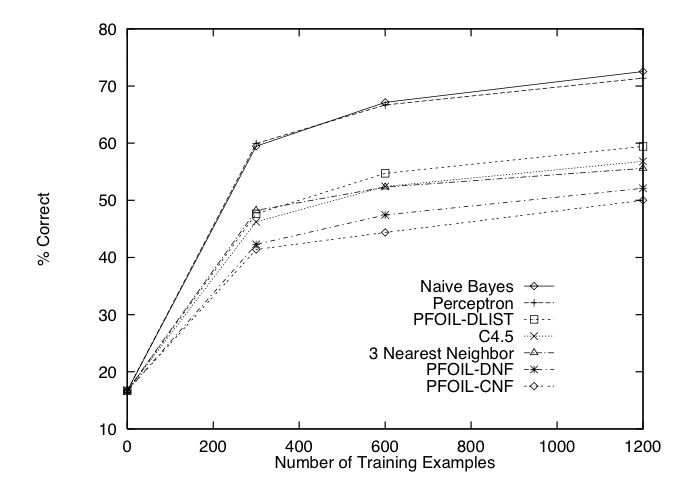
\includegraphics[keepaspectratio=true,
 width=0.9\columnwidth]{line_wsd_1_accuracy.png}
\caption{Рост точности решения WSD задачи для разных алгоритмов (определение значения слова \textit{line}) при увеличении размера обучающей выборки \cite{Mooney 1996}. Алгоритмы: PFOIL-DLIST, PROIL-DNF, PFOIL-CNF, C4.5, Naive Bayes --- наивный баейсовский классификатор; Perceptron --- персептрон; 3 Nearest Neighbor --- метод 3-х ближайших соседей}
\label{kor1}
\end{figure}

%Эксперименты учитывали не только точность определения значения, но и требовательность алгоритма к ресурсам в процессе обучения и работы. На %Рис.~\ref{kor2} можно увидеть зависимость времени обучения от размера выборки. Самыми быстрообучаемыми оказались байесовский классификатор и %перцептрон, а самыми медленными --- нормальные формы (Рис.~\ref{kor2}).

\begin{figure}[H]
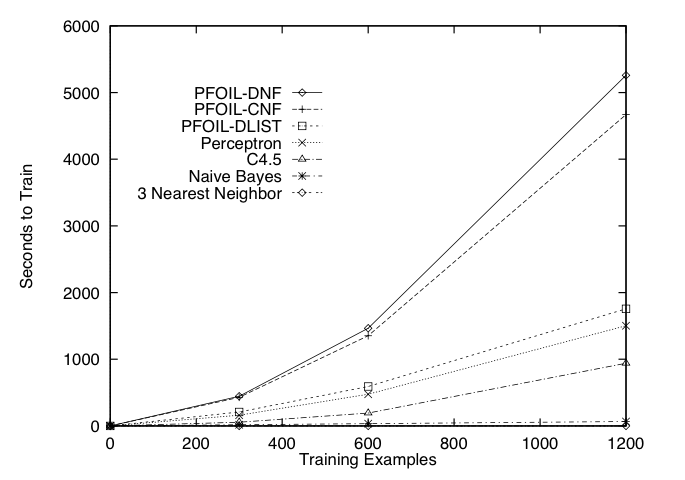
\includegraphics[keepaspectratio=true,
 width=0.9\columnwidth]{line_wsd_2_time.png}
\caption{Зависимость времени затраченного на обучение алгоритмов от размера обучающей выборки \cite{Mooney 1996}. Алгоритмы: PFOIL-DLIST, PROIL-DNF, PFOIL-CNF, C4.5, Naive Bayes --- наивный баейсовский классификатор; Perceptron --- персептрон; 3 Nearest Neighbor --- метод 3-х ближайших соседей}
\label{kor2}
\end{figure}

На Рис.~\ref{kor3} представлена зависимость времени работы алгоритмов от размера обучающей выборки. Время работы алгоритмов дает другую картину: байесовский классификатор и перцептрон работают долго при максимальном размере обучающей выборки, в то время как остальные методы решают WSD задачу за постоянное время (Рис.~\ref{kor3}). 

\begin{figure}[H]
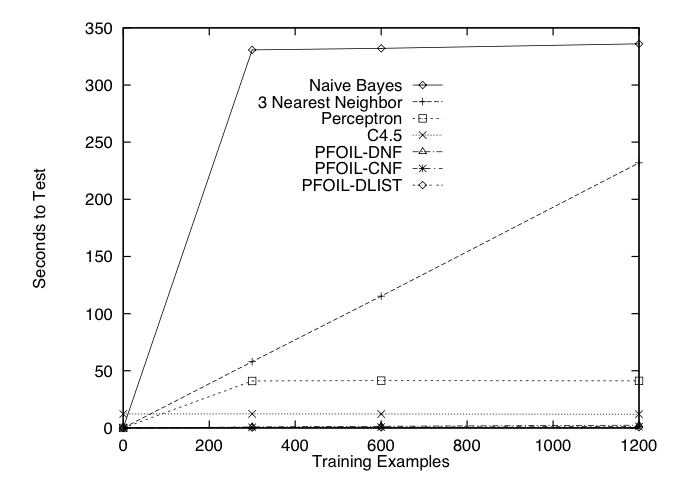
\includegraphics[keepaspectratio=true,
 width=0.9\columnwidth]{line_wsd_3_testing_time.png}
\caption{Зависимость времени работы алгоритмов от размера обучающей выборки при определении значения слова \textit{line} \cite{Mooney 1996}. Алгоритмы: PFOIL-DLIST, PROIL-DNF, PFOIL-CNF, C4.5, Naive Bayes --- наивный баейсовский классификатор; Perceptron --- персептрон; 3 Nearest Neighbor --- метод 3-х ближайших соседей}
\label{kor3}
\end{figure}

\bfullwidth
\begin{center}
\section{WSD-методы без учителя}
\end{center}
\efullwidth


\section{Различение значений слов на основе векторов свойств, расширенных словарными толкованиями}

\begin{flushright}
\textit{А. М. Спиркова} 
\end{flushright}

Амрута Пурандаре и Тед Педерсен в 2004 году разработали <<Алгоритм различения значений на основе контекстных векторов>> (\textit{Сontext vector sense discrimination}) \cite{Purandare 2004}. В этом алгоритме (1) берется набор примеров употреблений исследуемого слова, (2) выполняется кластеризация этих примеров так, чтобы близкие по значению или связанные каким-либо образом слова объединились в одну группу \cite{Purandare 2004}.
\parindent=0,5cm

\textit{Word sense discrimination} --- это задача группировки нескольких употреблений данного слова в кластеры, где каждому кластеру соответствует определенное значение целевого слова. Подходы к решению этой проблемы основываются на дистрибутивной гипотезе, которая говорит о том, что: лингвистические единицы, встречающиеся в схожих контекстах, имеют близкие значения. Следует различать понятия \textit{различение значений слов} и \textit{разрешение лексической многозначности}. При \textit{различении значений слов} нет никаких предопределенных значений слова, присоединенных к кластерам; здесь, скорее, слова, употребляющиеся в схожих контекстах, группируются в кластеры (значения).
\parindent=0,5cm

При решении задачи \textit{различения значений} используются контекстные вектора: если целевое слово встречается в тестовых данных, то контекст этого слова представляется в виде вектора контекста. \textit{Вектор контекста} --- это средний вектор по векторам свойств каждого из слов контекста. \textit{Вектор свойств} содержит информацию о совместной встречаемости данного слова с другими словами, этот вектор строится по данным корпуса текстов на этапе обучения.
\parindent=0,5cm

Метод различения значений Пурандаре и Педерсена \cite{Purandare 2004} предназначен для работы при недостаточном объеме текстовых данных, при этом вектор свойств расширяется данными, извлеченными из толкований словарей.
\parindent=0,5cm
Этот метод группирует в кластеры близкие по значению употребления целевого слова.
\parindent=0,5cm

\textbf{Построение матрицы встречаемости слов.} Первоначально строится матрица совместной встречаемости слов по данным обучающего корпуса (были использованы тексты Wall Street Journal и Британского национального корпуса).
\parindent=0,5cm

Вектор свойств (строка матрицы) содержит информацию о совместной встречаемости данного слова с другими. Было решено в \cite{Purandare 2004}, что слова <<встречаются>>, если они находятся в тексте на расстоянии не более пяти словопозиций (то есть между ними находится не более трех слов). 
\parindent=0,5cm

\textbf{Обработка матрицы.} После создания матрицы выполняется разделение тестовых данных, то есть группировка примеров употреблений (фраз) с целевым словом. Каждому слову в примере употребления  в тестовых данных соответствует вектор свойств из матрицы встречаемости. Средний вектор свойств по всем словам соответствует вектору контекста. Таким образом, набор тестовых данных, включающих употребление исследуемого слова, преобразуется в набор контекстных векторов, каждый из которых соответствует одному из употреблений целевого слова.
\parindent=0,5cm

Различение значений происходит путем кластеризации контекстных векторов с помощью разделяющего (partitional) или иерархического <<сверху вниз>> (agglomerative) алгоритма кластеризации \cite{Jain 1999}, \cite{Jain 1988}, \cite{Zhao 2002}.  Получающиеся кластеры составлены из употреблений близких по значению фраз, и каждый кластер соответствует отдельному значению целевого слова. 
\parindent=0,5cm

\textbf{Векторы свойств, расширенные текстами толкований из словаря.} Векторы свойств, полученные по небольшому корпусу текстов, имеют очень малую размерность (несколько сотен), что не позволяет полностью описать закономерности совместной встречаемости слов. Для решения этой проблемы векторы свойств слов расширяются содержательными словами (content words), извлеченными из словарных толкований разных значений данного слова. В Табл.~\ref{tbl2} представлены примеры толкований и содержательные слова для восьми значений слова <<история>> из Русского Викисловаря.

\bfullwidth
\begin{table}[H]
\centering
\caption{Словарные толкования (и содержательные слова) по данным статьи <<история>> из Русского Викисловаря. Серым цветом и курсивом выделены те слова, которые уже были в векторе слов, черным – новые слова из толкований, которыми будет расширен вектор свойств}
\begin{tabular}{|c|m{10cm}|m{5cm}|}

\hline
№ & Текст значения & Содержательные слова\\
\hline
1 & закономерное, последовательное развитие, изменение действительности & \textit{\textcolor{gray}{развитие,}} изменение\\
\hline
2 & наука, изучающая факты, тенденции и закономерности развития человеческого общества & \textit{\textcolor{gray}{наука,}} факт, тенденция, закономерность\\
\hline
3 & наука, изучающая ход развития, последовательные изменения какой-либо области природы или культуры & \textit{\textcolor{gray}{наука, развитие,}} изменение\\
\hline
4 & последовательный ход развития, изменения чего-либо, совокупность фактов о развитии какого-либо явления & \textit{\textcolor{gray}{развитие,}} изменение, факт\\
\hline
5 & отдаленное время с его событиями, происшествиями; прошлое & время, событие, происшествие\\
\hline
6 & эпическое повествование, рассказ & повествование, \textit{\textcolor{gray}{рассказ}}\\
\hline
7 & смешная или неожиданная ситуация, происшествие, случай & ситуация, случай, происшествие\\
\hline
8 & скандал, неприятность & скандал, неприятность\\
\hline
\end{tabular}
\label{tbl2}
\end{table}
\efullwidth

\parindent=0,5cm

Предположим, например, что вектор свойств (столбец в матрице встречаемости) для слова \textit{история} имеет непустые значения в строках, соответствующих словам: \textit{книга, мир, наука, образование, развитие, рассказ.}
\parindent=0,5cm 

В Русском Викисловаре различные значения слова \textit{история} (Табл.~\ref{tbl2}) включают содержательные слова: \textit{время, закономерность, изменение, наука, неприятность, повествование, происшествие,} развитие, рассказ, \textit{ситуация, скандал, случай, событие, тенденция, факт.} Таким образом, вектор свойств, соответствующий слову <<история>>, будет расширен новыми (отсутствующими ранее) словами из словаря: \textit{время, закономерность, изменение, неприятность, повествование, происшествие, ситуация, скандал, случай, событие, тенденция, факт.}
\parindent=0,5cm

В итоге, вектор свойств будет включать слова: \textit{время, закономерность, изменение,} книга, мир, наука, \textit{неприятность,} образование, \textit{повествование, происшествие,} развитие, рассказ, \textit{ситуация, скандал, случай, тенденция, факт.}
\parindent=0,5cm

Для оценки результатов тестовым примерам употребления присваивали вручную теги значений. Кластеру присваивалось то значение, примеров употребления которого в нем было больше всего. 
\parindent=0,5cm

Авторами было проведено 75 экспериментов с использованием 72 слов из корпуса SENSEVAL-2 и со словами \textit{line, hard} и \textit{serve.}
\parindent=0,5cm

В тестовых данных SENSEVAL-2 примеры употреблений включали 2-3 предложения. Для каждого слова было дано от 50 до 200 примеров употреблений в тестовых и тренировочных данных. Для этих слов известно много (порядка 8-12) значений. Малое число примеров при большем числе значений привело к тому, что для некоторых значений оказалось мало примеров употреблений. 43 из 72 слов SENSEVAL-2 показали улучшение F-меры и полноты (recall) при расширении вектора свойств текстами толкований словаря. Однако для 29 слов F-мера стала хуже, что, возможно, говорит о трудностях и несовершенстве метода. Для окончательной оценки необходима большая экспериментальная база: не десятки слов, а десятки и сотни тысяч.
\parindent=0,5cm

Данный метод может быть полезен при различении  значений слов без учителя при небольшом количестве обучающих данных.

\section{Автоматический поиск и кластеризация похожих слов}

\begin{flushright}
\textit{Д. С. Шорец} 
\end{flushright}

В работе \cite{Dekang 1998} представлена методология автоматического создания тезауруса, основанная на анализе корпуса текста и вычислении сходства слов, близости их значений. Значение незнакомого слова часто можно определить по контексту \cite{Eugene 1975}.  Рассмотрим, например, следующий текст:
\begin{flushright}
(1)\textit{Бутылка Tezg\"uino стоит на столе. Всем нравится Tezg\"uino. Tezg\"uino может привести к опьянению. Мы делаем Tezg\"uino из зерна.} 
\end{flushright}

Из этого контекста можно предположить, что \textit{Tezg\"uino} --- это алкогольный напиток, приготовленный из зерна.

Задача поиска похожих слов \textit{(similar words)} является первым шагом в определении значения слова. Тогда при обработке корпуса, включающего предложение (1), результатом должно быть определение близости значения слова \textit{Tezg\"uino} к словам \textit{пиво, вино, водка.}

\textbf{Методология автоматического создания тезауруса.} Для вычисления сходства между словами в работе \cite{Dekang 1998} использован парсер \cite{Dekang 1993}, извлекающий тройки из текста. Тройки зависимостей (от англ. \textit{dependency triple}, далее просто \textit{тройки}) состоят из двух слов и грамматического отношения между ними. Символ $||w, r, w'||$ означает частоту в корпусе тройки $(w, r, w')$, где $w, w'$ --- это слова в нормальной форме, $r$ --- синтаксическое отношение. Произвольное слово или отношение обозначается символом-джокером «*». Например, ||\textit{cook, obj,} *|| означает число троек со словом \textit{cook} и отношением \textit{obj}. 

Например из предложения \textit{<<У меня есть коричневая собака>>} будут извлечены следующие тройки:

\begin{center}
||\textit{коричневый, прил\_сущ, собака}||\\
||\textit{есть, гл\_сущ, собака}|| 
\end{center}

Определим следующие моменты:
\begin{enumerate} 
\item \textit{Описание слова w} --- это частоты всех троек ($w$, *, *) в корпусе,  то есть всех троек, включающих $w$. Описание слова $w$ является вектором.
\item \textit{<<Пересечение>> двух слов} --- это тройки, представленные в описании обоих слов; это пересечение векторов.
\end{enumerate}

Сходство между двумя объектами вычисляется как количество информации в <<пересечении>> двух объектов (2), деленное на количество информации в описании двух объектов (1), далее обозначено как функция \textit{sim($w_1, w_2$)} \cite{Dekang 1997}.

Предположив, что частоты троек не зависят друг от друга, получаем, что информация, представленная в описание слова $w$, равна сумме информации по каждой из уникальных троек в описании слова $w$. 

Для измерения информации в утверждении ||\textit{w, r, w'}||\textit{=с} выполним следующее:

\begin{enumerate}
\item измерим количество информации в утверждении, что произвольная тройка, извлеченная из текста, будет наша тройка \textit{(w, r, w')} при условии, что значение ||\textit{w, r, w'}|| --- не известно;
\item измерим то же при условии, что значение ||\textit{w, r, w'}|| --- известно;
\item разница этих двух количеств является ответом.
\end{enumerate}

Вероятность встретить в тексте тройку \textit{(w, r, w')} можно рассматривать как одновременное возникновение трех событий:

\textbf{A:} случайно выбранное слово - это $w$;

\textbf{B:} случайно выбранное отношение- это $r$;

\textbf{C:} случайно выбранное слово - это $w'$;

\begin{enumerate}
\item Когда значение ||\textit{w, r, w'}|| неизвестно, то предполагаем, что \textbf{А} и \textbf{С} являются условно независимыми при наличии события \textbf{В}.  Вероятность наступления сразу трех этих событий составляет \textbf{$P_{MLE}(B) P_{MLE} (A|B) P_{MLE} (C|B)$}, где \textbf{$P_{MLE}$} --- это оценка максимального правдоподобия распределения вероятностей (\textit{maximum likelihood estimation})

$P_{MLE}(B)=\frac{\displaystyle ||*,r,*||}{\displaystyle ||*,*,*||}$\\
$P_{MLE}(A|B)=\frac{\displaystyle ||w,r,*||}{\displaystyle ||*,r,*||}$\\
$P_{MLE}(C|B)=\frac{\displaystyle ||*,r,w'||}{\displaystyle ||*,r,*||}$

\item Когда значение ||\textit{w, r, w’}|| известно, можно сразу получить $P_{MLE}(A,B,C)$:

$P_{MLE}(A,B,C)=\frac{\displaystyle ||w,r,w'||}{\displaystyle ||*,*,*||}$
\item Пусть \textit{\textbf{I(w,r, w’)}} обозначает количество информации, содержащейся 
в утверждении ||\textit{w, r, w'}||\textit{=с}. Можно вычислить это значение так:
\end{enumerate}

%\bfullwidth
%\begin{center}
$$
I(w,r,w’)=
$$
$$
=-log(P_{MLE}(B) P_{MLE} (A|B) P_{MLE} (C|B))-
$$
$$
-(-log(P_{MLE}(A,B,C))=
$$
$$
=log\frac{||w,r,w'||\times||*,r,*||}{||w,r,*||\times||*,r,w'||}.
$$

%$\end{center}
%$\efullwidth

Отметим, что значение \textit{I(w,r,w’)} равно количеству взаимной информации (\textit{mutual information}) между $w$ и $w'$ \cite{Donald 1990}.

Пусть $T(w)$ --– это множество пар \textit{(r, w')}, при которых $log\frac{\displaystyle ||w,r,w'||\times||*,r,*||}{\displaystyle ||w,r,*||\times||*,r,w'||}$ имеет положительное значение. Определим значение сходства (похожести) двух слов \textit{w1} и \textit{w2} с помощью формулы:

%\bfullwidth
%\begin{center}
$$
sim(w_1,w_2)=
$$
$$
\frac{\displaystyle \sum_{(r,w)\in T(w_1)\cap T(w_2)}(I(w_1,r,w)+I(w_2,r,w))}{\displaystyle \sum_{(r,w)\in T(w_1)}I(w_1,r,w)+\sum_{(r,w)\in T(w_2)}I(w_2,r,w)}.
$$
%\end{center}
%\efullwidth

\textbf{Практическая реализация метода.} Был обработан корпус, включающий 64 млн. слов. Из него было извлечено 56,6 миллионов троек, включающих 8,7 миллиона уникальных троек.

Сам корпус был разбит на классы по частям речи.  Исследовалось попарно сходство между всеми глаголами, всеми существительными, всеми прилагательными/наречиями по формуле $sim(w_1 , w_2)$. Для каждого слова был построен аналог словарной статьи в тезаурусе, включающий упорядоченный набор 200 наиболее похожих слов. Статья в тезаурусе для слова $w$ имела следующий формат:\\

$w(pos):w_1,s_1,w_2,s_2,\ldots,w_N,s_N$\\

где \textit{pos} --– это часть речи, $w_i$ ---  это похожее слово, $s_i$ --- это значение сходства между $w$ и $w_i$, слова упорядочены по убыванию значения сходства.

Два слова являются \textit{парой взаимных ближайших соседей (RNN от respective nearest neighbors)}, если они являются наиболее похожими словами друг для друга (первыми в списке из двухсот слов). С помощью программы удалось получить 543 пары RNN существительных, 212 пар RNN глаголов, 382 пары RNN прилагательных/наречий в созданном автоматически тезаурусе. В Табл.~\ref{tabshor} представлен список каждого 10-го RNN для глаголов.

\bfullwidth
\begin{table}[H]
\centering
\caption{Список пар взаимных ближайших соседей (RNN) глаголов}
\begin{tabular}{|c|c|c|}
\hline
\textbf{Ранг} & \textbf{RNN} & \textbf{Значение сходства}\\
\hline
1 & \textit{fall rise} & 0,67\\
\hline
11 & \textit{injure kill} & 0,38\\
\hline
21 & \textit{concern worry} & 0,34\\
\hline
31 & \textit{convict sentence} & 0,29\\
\hline
41 & \textit{limit restrict} & 0,27\\
\hline
51 & \textit{narrow widen} & 0,26\\
\hline
61 & \textit{attract draw} & 0,24\\
\hline
71 & \textit{discourage encourage} & 0,23\\
\hline
81 & \textit{hit strike} & 0,22\\
\hline
91 & \textit{distregard ignore} & 0,21\\
\hline
101 & \textit{overstate understate} & 0,20\\
\hline
111 & \textit{affirm reaffirm} & 0,18\\
\hline
121 & \textit{inform notify} & 0,17\\
\hline
131 & \textit{differ vary} & 0,16\\
\hline
141 & \textit{scream yell} & 0,15\\
\hline
151 & \textit{laugh smile} & 0,143\\
\hline
161 & \textit{compete cope} & 0,136\\
\hline
171 & \textit{add whisk} & 0,130\\
\hline
181 & \textit{blossom mature} & 0,12\\
\hline
191 & \textit{smell taste} & 0,11\\
\hline
201 & \textit{bark howl} & 0,10\\
\hline
211 & \textit{black white} & 0,07\\
\hline
\end{tabular}
\label{tabshor}
\end{table}
\efullwidth

\section{Разрешение многозначности в биомедицинских текстах с помощью методов кластеризации без учителя}

\begin{flushright}
\textit{Е. А. Ярышкина} 
\end{flushright}

В статье \cite{Savova 2005} изучаются уже существующие методы кластеризации без учителя и их эффективность для решения лексической многозначности при обработке текстов по биомедицине. Решение проблем лексической многозначности в данной области включает в себя не только традиционные задачи присвоения ранее определенных смысловых значений для терминов, но так же и обнаружения новых значений для них, еще не включенных в данную онтологию.
\parindent=0,5cm

Авторы описали методологию способа разрешения лексической многозначности без учителя, учитываемые лексические признаки и наборы экспериментальных данных. В качестве оценки эффективности алгоритмов кластеризации текста была предложена F-мера. 
\parindent=0,5cm

Подход для решения поставленной задачи --- это разделение контекстов (фрагментов текста), содержащих определенное целевое слово, на кластеры, где каждый кластер представляет собой различные значения целевого слова. Каждый кластер состоит из близких по значению контекстов. Задача решается в предположении, что используемое целевое слово в аналогичном контексте будет иметь один и тот же или очень похожий смысл. 
\parindent=0,5cm

Процесс кластеризации продолжается до тех пор, пока не будет найдено предварительно заданное число кластеров. В данной статье выбор шести кластеров основан на том факте, что это больше, чем максимальное число возможных значений любого английского слова, наблюдаемое среди данных (большинство слов имеют два-три значения). Нормализация текста не выполняется.
\parindent=0,5cm

Данные в этом исследовании состоят из ряда контекстов, которые включают данное целевое слово, где у каждого целевого слова вручную отмечено --- какое значение из словаря было использовано в этом контексте. Контекст --- это единственный источник информации о целевом слове. Цель исследования --- преобразовать контекст в контекстные вектора первого и второго порядка \cite{epr:website}. Контекстные вектора содержат следующие «лексические свойства»: биграммы, совместную встречаемость и совместную встречаемость целевого слова. Биграммами являются как двухсловные словосочетания, так и любые два слова, расположенные рядом в некотором тексте. Для лингвистических исследований могут быть полезны только упорядоченные наборы биграмм \cite{Averin 2006}. 
\parindent=0,5cm

Экспериментальные данные --- это набор NLM WSD \cite{UMLS:website} (NLM --- национальная библиотека медицины США), в котором значения слов взяты из UMLS (единая система медицинской терминологии). UMLS имеет три базы знаний: 
\begin{itemize}
\item Метатезаурус включает все термины из контролируемых словарей (SNOMED-CT, ICD и другие) и понятия, которые представляют собой кластера из терминов, описывающих один и тот же смысл. 
\item Семантическая сеть распределяет понятия на 134 категории и показывает отношения между ними. SPECIALIST-лексикон содержит семантическую информацию для терминов Метатезауруса. 
\item Medline --- главная библиографическая база данных NLM, которая включает приблизительно 13 миллионов ссылок на журнальные статьи в области науки о жизни с уклоном в биомедицинскую область.
\end{itemize}
\parindent=0,5cm

Авторы успешно проверили по три конфигурации существующих методов (PB --- Pedersen and Bruce \cite{Pedersen 1997}, SC --- Sch\"utze \cite{Schutze 1998}) и оценили эффективность использования SVD (сингулярное разложение матриц). Методы PB основаны на контекстных векторах первого порядка --- признаки одновременного присутствия целевого слова или биграммы. Рассчитывается среднее расстояние между кластерами или применяется  метод бисекций. PB методы подходят для работы с довольно большими наборами данных. Методы SC основаны на представлениях второго порядка --- матрицы признаков одновременного присутствия или биграммы, где каждая строка и столбец --- вектор признаков первого порядка данного слова. Так же рассчитывается среднее расстояние между кластерами или применяется  метод бисекций. SC методы подходят для обработки небольших наборов данных.  

\parindent=0,5cm
Метод SC2 (признаки одновременного присутствия второго порядка, среднее расстояние между элементами кластера в пространстве подобия) с применением и без SVD показал лучшие результаты: всего 56 сравниваемых экземпляров, в 47 случаях метод SC2 показал наилучшие результаты, в 7 случаях результаты незначительно отличаются от других проверяемых методов.
\parindent=0,5cm

Все эксперименты, указанные в исследовании, выполнялись с помощью пакета SenseClusters \cite{SC:website}. В ходе исследования было проведено два эксперимента для разных наборов данных. Маленький тренировочный набор --- это набор NLM WSD, который включает 5000 экземпляров для 50 часто встречаемых неоднозначных терминов из Метатезауруса UMLS. Каждый неоднозначный термин имеет по 100 экземпляров с указанным вручную значением. У 21 термина максимальное число экземпляров находится в пределах от 45 до 79 экземпляров. У 29 терминов число экземпляров от 80 до 100 для  конкретного значения. Стоит отметить, что каждый термин имеет категорию «ни одно из вышеупомянутых», которая охватывает все оставшиеся значения, не соответствующие доступным в UMLS. Большой тренировочный набор является реконструкцией «1999 Medline», который был разработан Weeber \cite{Weeber 2001}. Были определены все формы из набора NLM WSD и сопоставлены с тезисами «1999 Medline». Для создания тренировочного набора экземпляров использовались только те тезисы из «1999 Medline», которым было найдено соответствие в наборе NLM WSD.
\parindent=0,5cm

Использование целиком текста аннотации статьи в качестве контекста приводит к лучшим результатам, чем использование отдельных предложений. С одной стороны, большой объем контекста, представленный аннотацией, дает богатую коллекцию признаков, с другой стороны, в коллекции WSD представлено небольшое число контекстов.

\section{Выявление значений слов из текста}
\begin{flushright}
\textit{Д. Ю. Янкевич} 
\end{flushright}

В статье \cite{Pantel 2002} представлен алгоритм автоматического обнаружения значений слов в тексте, названный \textit{кластеризация посредством комитетов} (Clustering By Committee (CBC)). Также авторы предлагают методологию оценки для автоматического измерения точности и полноты найденных значений.
\parindent=0,5cm

\textbf{Алгоритм} первоначально находит множество небольших кластеров, называемых комитетами, каждый из которых представляет собой одно из значений определяемого слова. Центр тяжести  членов комитета (мера связности с определяемым словом) используется в качестве вектора признаков кластера.
\parindent=0,5cm

CBC состоит из трех этапов.
\parindent=0,5cm

На этапе I для каждого элемента (слова) вычисляются $k$ наиболее похожих слов. Сначала весь список относящихся к слову значений сортируется по убыванию значений связи согласно формуле точечной взаимной информации (pointwise mutual information (PMI) \cite{Manning 1999}), а затем, с помощью иерархического кластерного анализа по \textit{методу средней связи} \cite{Kim 1989}, вычисляется сходство между всеми элементами кластера попарно. Значение функции PMI \cite{Manning 1999} между предполагаемым значением слова (контекстом) и элементом (словом) вычисляется следующим образом: пусть x --- это рассматриваемый элемент, а y --- контекст. \textit{Точечная взаимная информация} между x и y определена как:

$$
pmi(x;y)\equiv log \frac{\displaystyle p(x,y)}{\displaystyle p(x)p(y)}=
$$
$$
=log\frac{\displaystyle p(x|y)}{\displaystyle p(x)}=log\frac{\displaystyle p(y|x)}{\displaystyle p(y)}.
$$
\parindent=0,5cm

При кластеризации посредством метода средних связей \textit{(average-link clustering)} вычисляется среднее сходство между данным объектом и всеми объектами в кластере, а затем, если найденное \textit{среднее значение сходства} достигает или превосходит некоторый заданный пороговый уровень сходства, объект присоединяется к этому кластеру \cite{Kim 1989}. Сложность этого алгоритма $O(n^2 * log (n))$, где $n$ --- число кластеризуемых элементов \cite{Jain 1999}.
\parindent=0,5cm

В этапе I оценка (PMI) означает предпочтение большим и тесно связанным кластерам.
\parindent=0,5cm

На II этапе строится набор небольших кластеров, где элементы каждого кластера образуют комитет. В ходе работы <<Алгоритма~1>> формируется как можно больше комитетов при условии, что каждый вновь созданный комитет не слишком похож на любой из уже существующих комитетов. Если условие нарушается, комитет просто отбрасывается. Алгоритм описан ниже подробно.

\bfullwidth
\begin{algorithm}[H]
\SetAlgoLined
\KwData{Список элементов $E$, которые будут сгруппированы, база данных сходства $S$, из фазы I, пороги $\theta1$ и $\theta2$ (с помощью порога $\theta1$ сохраняются только те кластеры, которые имеют значения, отличные от ранее обнаруженных, порог $\theta2$ позволяет обнаружить элементы, не принадлежащие ни одному из кластеров)}
\KwResult{$C$ --- список комитетов}
\textbf{Step 1:}\\
\ForEach{$e \in E$}{\begin{enumerate}
\item Кластер k наиболее <<близких>> (похожих) элементов е из S с помощью метода  средней связи
\item Для каждого обнаруженного кластера $c$ вычислить следующую оценку:
$val = | C | * avgsim(c)$, где $| C |$ --- количество элементов $c$ и $avgsim(c)$ --- усредненное сходство между всеми парами элементов кластера $c$.
\item Записать кластер с наивысшей оценкой в список $L$\end{enumerate}}
\textbf{Step 2:}\\
Сортировка кластеров в списке $L$ в порядке убывания их оценок $val$\\
\textbf{Step 3:}\\
$C = \emptyset$ // Пусть $C$ перечень комитетов, изначально пустой\\
\ForEach{$c \in L$}{// в отсортированном по убыванию порядке:
\begin{enumerate}
\item Вычислить центр тяжести, усредняя поэлементно значение векторов, и вычислить вектор  PMI центроида (точно так же, как мы делали для отдельных элементов)
\item Если схожесть $c$ и центроида каждого комитета, ранее добавленного к $C$, ниже порогового $\theta1$, то следует добавить $c$ в $C$
\end{enumerate}}
\textbf{Step 4:}\\
\If{$C=\emptyset$}{\Return $C$}
$R = \emptyset$ // $R$ --- это множество остатков, то есть элементов, не охваченных ни одним из кластеров\\
\ForEach{$e \in E$}{\ForEach{$c \in C$}{\If{$sim(e, c) < \theta2$ // $sim(e,c)$ --- схожесть $e$ каждому комитету из $C$}{$R += e$ // то следует добавить $e$ в список остатков $R$}}}
\If{$R=\emptyset$}{\Return $C$ \Else{\Return $C \cup Algorithm1(R, S, \theta1, \theta2)$}}
\caption{II фаза кластеризации посредством комитетов (CBC)}
\label{alg}
\end{algorithm}
\efullwidth

В результате второго этапа построения CBC остаются кластеры, связанные более тесно (имеющие большее значение val, см. step 1 и 3 алгоритма~\ref{alg}).
\parindent=0,5cm

На заключительном III этапе работы алгоритма каждый элемент e присваивается наиболее подходящему кластеру следующим образом (при этом центроид членов комитета используется в качестве вектора характеристик кластера):

\bfullwidth
\begin{algorithm}[H]
\SetAlgoLined

\KwResult{Итоговые кластеры с максимальным значением связи (val) между словами}
Пусть $С$ список кластеров (изначально пустых)\\
Пусть $S$ это топ-200 кластеров, схожих с $e$\\
\While{$S$ не пуст}{пусть $c \in S$ наиболее близкий кластер к $e$\\
\If{сходство $(e, c) < \sigma$}{\textbf{конец цикла}}
\If{$c$ не схож ни с одним кластером в $C$}{присвоить $e$ к $c$\\
удалить из $e$ его характеристики, которые перекрываются с характеристиками $c$}
удалить $c$ из $S$
}
\caption{Присвоение элементов кластерам}
\label{alg1}
\end{algorithm}
\efullwidth

На III этапе кластер сохраняется только в случае, если его сходство со всеми ранее полученными кластерами ниже установленного порогового значения.
\parindent=0,5cm

Согласно дистрибутивной гипотезе (Distributional Hypothesis) \cite{Harris 1985} слова, употребляемые в сходных контекстах, близки по смыслу. Алгоритм \textit{Кластеризации посредством комитетов} \cite{Pantel 2002} разрешает лексическую многозначность, группируя слова согласно сходству их контекстов. Каждому полученному кластеру соответствует одно из значений слова.
\parindent=0,5cm

%В Табл.~\ref{yank} каждая запись показывает кластеры, которым принадлежит заглавное слово. Имена для кластеров Nq34, Nq137, $\ldots$ генерируются %автоматически. После каждого имени кластера находится число, обозначающее сходство между кластером и заглавным словом (т.е. рукав, сердце и одежда). %Далее перечисляются четыре слова, наиболее близкие центроиду кластера. Каждый кластер соответствует одному значению заглавного слова. Например, Nq34 %соответствует значению <<деталь одежды>>, а Nq137 соответствует значению <<ответвление русла реки>>.

\begin{table}[H]
\caption{Для построения кластеров использовались данные словарных статей Викисловаря: <<одежда>>,  <<рукав>> и  <<сердце>>}
\begin{tabular}{|c|c|m{5cm}|}
\hline
\multicolumn{3}{|c|}{Рукав}\\
\hline 
Nq34 & 0.39 & деталь, манжета, полотно\\
Nq137 & 0.20 & протока, русло, отмель, поток\\
Nq217 & 0.18 & шланг, труба, огнетушитель\\
\hline
\multicolumn{3}{|c|}{Сердце}\\
\hline
Nq72 &  0.27 & орган, костный мозг, почка\\
Nq866 & 0.17 & душа, рассудок, сознание\\
\hline
\multicolumn{3}{|c|}{Одежда}\\
\hline
Nq215 & 0.41 & мануфактура, юбка, брюки\\
Nq235 & 0.20 & покрытие, оболочка, дорога\\
\hline
\end{tabular}
\label{yank}
\end{table}

В Табл.~\ref{yank} каждая запись показывает кластеры, которым принадлежит заглавное слово. Имена для кластеров Nq34, Nq137, $\ldots$ генерируются автоматически. После каждого имени кластера находится число, обозначающее сходство между кластером и заглавным словом (т.е. рукав, сердце и одежда). Далее перечисляются четыре слова, наиболее близкие центроиду кластера. Каждый кластер соответствует одному значению заглавного слова. Например, Nq34 соответствует значению <<деталь одежды>>, а Nq137 соответствует значению <<ответвление русла реки>>.


\textbf{Сравнение с алгоритмом UNICON.} CBC является разновидностью алгоритма UNICON \cite{Lin 2001}, который также строит центроид кластера, используя небольшой набор похожих элементов.
\parindent=0,5cm

Одним из основных различий между UNICON и CBC является то, что UNICON гарантирует, что различные комитеты не имеют одинаковых элементов, тем не менее, центры тяжести двух комитетов по-прежнему могут быть очень близкими (похожими). В~UNICON'е эта проблема решается объединением таких кластеров. В отличие от этого, на II этапе CBC создаются только те комитеты, центры тяжести которых отличны от всех ранее созданных комитетов.
\parindent=0,5cm

Есть разница и на III этапе CBC. Алгоритм UNICON плохо работает со словами, которые имеют несколько широко используемых (доминирующих) значений. Например, пусть значение <<отмычка>> является более употребимым для слова <<ключ>>, чем значение <<водный источник>>. Приведем смесь слов-синонимов к разным значениям слова <<ключ>>: пневмоключ, электроключ, родник, родничок, источник, криница, гидроключ, ключик, тангента, треншальтер, тумблер, знак, контролька, отпирка, виброплекс, шифр. В этом списке 10 значений относятся к значению <<отмычка()>>, 4 к <<водный источник()>> и 2 к значению <<знак()>>. По этому списку алгоритмом UNICON будут сгенерированы кластеры <<отмычка>>, <<шифрование>>, <<происхождение>>,<<криптография>>, <<кнопка>>, <<водный источник>>,<<переключатель>>, <<намек>>. Сходство между словом и полученными кластерами  является очень низким, к тому же есть кластеры, содержащие одинаковые слова. С другой стороны, CBC удаляет <<пересекающиеся>> (общие для двух кластеров) характеристики после того, как присвоит значение кластеру (допустим характеристики, относящиеся к значению <<отмычка>> слова <<ключ>> из вектора характеристик <<отмычка>>). В результате, сходство между  кластером <<водный источник>> \{родник, родничок, источник, криница\} и пересмотренным вектором характеристик кластера <<водный источник>> становится намного выше. Что в свою очередь приводит к тому, что кластеры становятся гораздо точнее.

\bfullwidth
\begin{center}
\section{WSD-методы, основанные на знаниях}
\end{center}
\efullwidth

\section{Использование лексических цепочек для реферирования текстов}
\begin{flushright}
\textit{А. В. Пилинович} 
\end{flushright}

В статье \cite{Barzilay Elhadad 1997} с целью реферирования текста строится модель в виде лексических цепочек. Реферирование включает четыре этапа: оригинальный текст делится на блоки (сегменты), строятся лексические цепочки, определяются сильные цепочки, извлекаются важные предложения.

Реферирование --- это процесс сжатия исходного текста в более компактный, при сохранении информативности текста. Реферирование выполняется для решения разных задач - от обзорного анализа текстов какой-либо научной области до быстрого выделения главных тем текста. Создание качественной информативной аннотации произвольного текста является сложной задачей, требующей полного понимания текста. Легче создавать  приблизительные, указательные аннотации (indicative summaries), позволяющие принять решение --- стоит ли читать текст. В работе \cite{Barzilay Elhadad 1997} описан метод создания указательных аннотаций по произвольным текстам.

Интуитивное понятие \textit{cohesion} (связность, склеивание, слияние), введенное в \cite{Halliday Hasan 1976}, указывает на объединение разных частей (фрагментов) текста в одно целое, в то, что имеет значение, смысл. Одним из видов связности является \textit{лексическая связность} (lexical cohesion) \cite{Hoey 1991}. Лексическая связность формируется с помощью семантически связанных слов. Halliday и Hasan \cite{Halliday Hasan 1976} выделили  два способа формирования лексической связности: (1) с помощью категории повторений и (2) категории словосочетаний. 

\begin{enumerate} 
\item \textit{Лексическая связность повторений} (reiteration category) достигается повтором слов, использованием синонимов и гипонимов. 
\item \textit{Лексическая связность словосочетаний} (collocation category) определена для слов, которые часто употребляются вместе, то есть встречаются в одних и тех же контекстах.
\end{enumerate}

Слова и фразы, между которыми существует лексическая связность, формируют лексическую цепочку (lexical chains) \cite{Hoey 1991}. Метод лексических цепочек, предложенный Барзилей и Эльхадад \cite{Barzilay Elhadad 1997}, основан на анализе совместной встречаемости слов и лексических связей между словами. 

\textbf{Алгоритм построения цепочек.} Достоинство лексических цепочек в том, что их легко распознать и построить. Первая вычислительная модель для лексических цепочек была представлена в работе Морриса и Хирста \cite{Hoey 1991}. Цепочки создавались путем взятия нового слова из текста и поиска родственной (связанной) цепочки для слова в соответствии с критериями родства. Недостатком подхода в \cite{Hoey 1991} было то, что в одну цепочку могло входить слово с разными значениями (для многозначных слов). Таким образом, выбор подходящей цепочки для слова эквивалентен решению WSD-задачи.

Метод построения лексических цепочек включает шаги:

\begin{enumerate} 
\item Выбирается набор слов-кандидатов (существительные и составные существительные). Это кандидаты на включение в цепочки.
\item Строится список всех значений для каждого слова-кандидата (по данным словаря).
\item Для каждого значения каждого слова-кандидата находится (вычисляется) отношение (расстояние) до каждого слова во всех уже построенных цепочках (слово в цепочке имеет строго определённое значение, задаваемые другими словами в той же цепочке). Между двумя словами есть отношение (будет указана связь в цепочке), если мало расстояние между этими словами в тексте (text distance) или между значениями этих слов существует путь в тезаурусе WordNet. Выделяют три вида отношений (\cite{Do Thuy Duong 2011}, стр. 36):
\begin{enumerate} 
\item \textit{Extra-strong} отношение существует для слов, повторяющихся в тексте. Повтор может быть на любом расстоянии от первого употребления слова.
\item \textit{Strong} отношение определено между словами, связанными отношением в WordNet. Два таких слова должны находиться в окне не более семи предложений.
\item \textit{Medium-strong} отношение указывается для слов, синсеты которых находятся на расстоянии больше одного в WordNet (но есть ещё и дополнительные ограничения на путь между синсетами). Слова в тексте должны находиться в пределах трех предложений.
\end{enumerate} 
\item Слово-кандидат добавляется в цепочки, со словами которых найдена связь. Смысловая неоднозначность устраняется, то есть в цепочку добавляется не просто слово, а его конкретное значение (благодаря выбору значения в словаре на шаге 2).
\end{enumerate} 

Для выбора приоритетной цепочки, (для вставки слова-кандидата) отношения упорядочены так: extra-strong, strong, medium-strong. В работе Хирста и Ст-Онж \cite{Hirst St-Onge 1998} предложен жадный алгоритм выбора цепочек. При этом слово-кандидат попадает ровно в одну цепочку и после этого выбор уже не может быть изменён, даже если последующий текст покажет ошибочность первоначального решения. В работе Барзилей и Эльхадад \cite{Barzilay Elhadad 1997} предложена более сложная схема выбора <<подходящего значения>>, требующая рассмотрения всех возможных цепочек. Таким образом, будут сформированы цепочки с учетом всех возможных значений слов с последующим выбором наилучшей цепочки. Эта более сложная схема и рассматривается далее.

Для иллюстрации метода приводится пример на отрывке текста, представленном ниже, и посмотрим, какое значение будет выбрано для слова \textit{machine}. Во-первых, для слова \textit{Mr.} создается узел [лексема "Mr.", значение \{mister, Mr.\}]. Следующим по тексту существительным, представленным в тезаурусе WordNet, будет слово \textit{person}, у него есть два значения: \textit{“human being”} ($person_1$) и \textit{“grammatical category of pronouns and verb forms”} ($person_2$). Наличие двух значений у слова \textit{person} разбивает пространство цепочек на два множества интерпретаций: в первой интерпретации используется значение  $person_1$, во второй --- $person_2$, (Рис.~\ref{step1}).

\begin{figure}[H]
    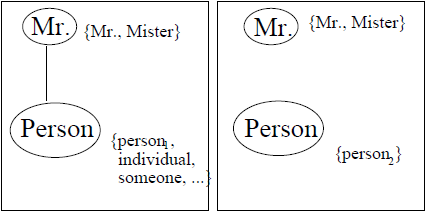
\includegraphics[keepaspectratio=true,width=0.9\columnwidth]{step_1_int_1_2.PNG}
    \caption{Шаг 1, интерпретация 1 и 2}
    \label{step1}
\end{figure}

\textit{\textbf{Mr.} Kenny is the \textbf{person} that invented an anesthetic \textbf{machine} which uses \textbf{micro-computers} to control the rate at which an anesthetic is pumped into the blood. Such \textbf{machines} are nothing new. But his \textbf{device} uses two \textbf{micro-computers} to achieve much closer monitoring of the \textbf{pump} feeding the anesthetic into the patient.}

\textit{Компонентой} в \cite{Barzilay Elhadad 1997}  называют список взаимоисключающих интерпретаций. Именно посредством компонент выбор одного из значений слов ведёт к выбору соответствующей интерпретации, а, следовательно, к невозможности других интерпретаций из этой компоненты. Интерпретации 1 и 2 на Рис.~\ref{step1} являются компонентой.

Следующее слово \textit{anesthetic} не связано со словами из первой компоненты, поэтому для него создается  компонента с одним значений (то есть новая компонента содержит ровно одну интерпретацию). 

Следующее слово \textit{machine} имеет 5 значений: от $machine_1$  до $machine_2$. В первом значении $machine_1$  [лексема "machine", значение \{an efficient person\}] слово связано со значениями слов $person$ и $Mr.$, поэтому слово $machine$  вставляется в первую компоненту. После этой вставки изображение первой компоненты становится таким, как показано на Рис.~\ref{step2}. Если продолжить этот процесс и вставить слова \textit{micro-computer, device} и \textit{pump,} то количество альтернативных вариантов значительно увеличивается. Самые сильные интерпретации представлены на Рис.~\ref{step6}. При условии, что текст связный, лучшей интерпретацией считается та, которая имеет больше всего связей. В данном  случае в конце шага 3 выбрана другая интерпретация $machine_4$ [лексема "machine", значение \{\textit{any mechanical or electrical device that performs or assists in the performance}\}], что верно отражает значение слова \textit{machine} в этом контексте.

%Оценка интерпретации определяется как сумма оценок ее цепочек. 
%Оценка цепочки определяется количеством и весом отношений между участниками цепочки. 
%В эксперименте авторы зафиксировали следующий вес: повторения и синонимы  --- 10, антонимы --- 7, 
%гиперонимы и гипонимы --- 4. Описанный алгоритм вычисляет все возможные интерпретации, 
%не допуская противоречий между ними. 
%Когда число возможных интерпретаций превышает определенный порог, слабые интерпретации удаляются, 
%это необходимо для предотвращения экспоненциального роста использования памяти.

\bfullwidth
\begin{figure}
        \centering
        \begin{subfigure}[b]{0.33\textwidth}
                \fbox{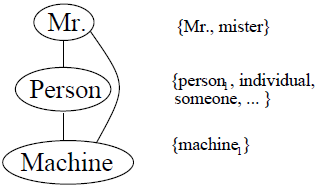
\includegraphics[width=\textwidth]{step_2_int_1.PNG}}
%                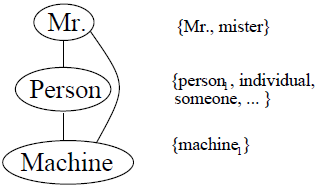
\includegraphics[width=\textwidth]{step_2_int_1.PNG}
%                \caption{Шаг 2, интерпретация 1}
                \caption{Интерпретация 1}
        \end{subfigure}%
%        \hfill%%% horizontal distance between two images (side by side)
        \quad% add desired spacing between images, e. g. ~, \quad, \qquad, \hfill etc.
             % (or a blank line to force the subfigure onto a new line)
        \begin{subfigure}[b]{0.39\textwidth}
                \fbox{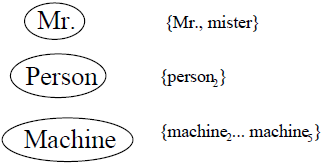
\includegraphics[width=\textwidth]{step_2_int_2.PNG}}
%                \caption{Шаг 2, интерпретация 2}
                \caption{Интерпретация 2}
        \end{subfigure}
\end{figure}
\efullwidth

\bfullwidth
\begin{figure}
        \centering
        %~ %add desired spacing between images, e. g. ~, \quad, \qquad, \hfill etc.
          %(or a blank line to force the subfigure onto a new line)
        \begin{subfigure}[b]{0.39\textwidth}
                \fbox{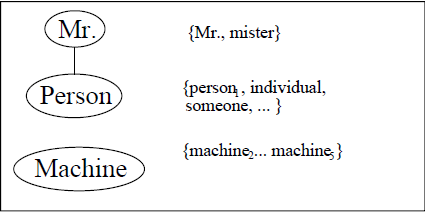
\includegraphics[width=\textwidth]{step_2_int_3.PNG}}
%                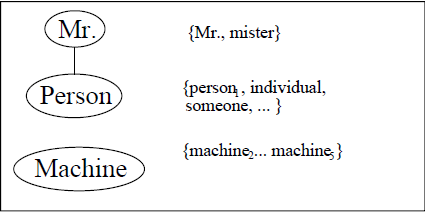
\includegraphics[width=\textwidth]{step_2_int_3.PNG}
%                \caption{Шаг 2, интерпретация 3}
                \caption{Интерпретация 3}
        \end{subfigure}
%        \hfill%%% horizontal distance between two images (side by side)
        \quad% add desired spacing between images, e. g. ~, \quad, \qquad, \hfill etc.
             % (or a blank line to force the subfigure onto a new line)
        \begin{subfigure}[b]{0.33\textwidth}
                \fbox{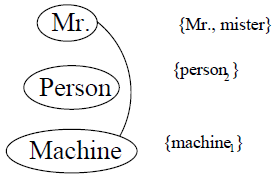
\includegraphics[width=\textwidth]{step_2_int_4.PNG}}
%                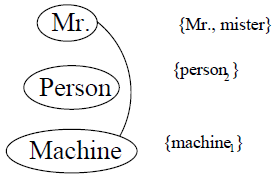
\includegraphics[width=\textwidth]{step_2_int_4.PNG}
%                \caption{Шаг 2, интерпретация 4}
                \caption{Интерпретация 4}
        \end{subfigure}
        \caption{Четыре интерпретации на втором шаге}\label{step2}
\end{figure}
\efullwidth

\bfullwidth
\begin{figure}
        \centering
        \begin{subfigure}[b]{0.42\textwidth}
                \fbox{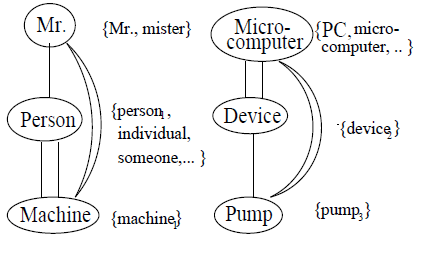
\includegraphics[width=\textwidth]{step_3_int_1.PNG}}
%                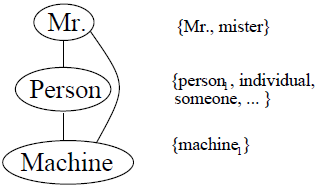
\includegraphics[width=\textwidth]{step_2_int_1.PNG}
%                \caption{Шаг 2, интерпретация 1}
                \caption{Интерпретация 1}
        \end{subfigure}%
        \quad% add desired spacing between images, e. g. ~, \quad, \qquad, \hfill etc.
             % (or a blank line to force the subfigure onto a new line)
        \begin{subfigure}[b]{0.42\textwidth}
                \fbox{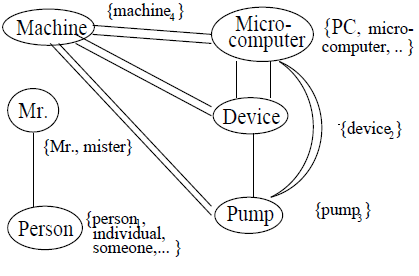
\includegraphics[width=\textwidth]{step_3_int_2.PNG}}
%                \caption{Шаг 2, интерпретация 2}
                \caption{Интерпретация 2}
        \end{subfigure}
        \caption{Две самые сильные интерпретации, полученные на третьем шаге}\label{step6}
\end{figure}
\efullwidth

Оценка интерпретации определяется как сумма оценок ее цепочек. 
Оценка цепочки определяется количеством и весом отношений между участниками цепочки. 
В эксперименте авторы зафиксировали следующий вес: повторения и синонимы  --- 10, антонимы --- 7, 
гиперонимы и гипонимы --- 4. Описанный алгоритм вычисляет все возможные интерпретации, 
не допуская противоречий между ними. 
Когда число возможных интерпретаций превышает определенный порог, слабые интерпретации удаляются, 
это необходимо для предотвращения экспоненциального роста использования памяти.


\textbf{Объединение цепочек из разных сегментов.} Текст предварительно разбивается на сегменты (несколько предложений или абзац). Пример выше (\textit{Mr. Kenny...}) соответствует одному сегменту. Цепочки строятся для каждого сегмента на основе найденных отношений между словами (extra-strong, strong, medium-strong). На следующем этапе объединяются цепочки из разных сегментов, но для объединения нужно, чтобы выполнялось еще более жесткое условие: две цепочки объединяются, если они содержат одно и то же слово в одном и том же значении. Поскольку есть прямая связь между цепочками и смысловыми блоками текста, постольку с помощью лексических цепочек можно решать и обратную задачу --- разбиение текста на сегменты \cite{Barzilay Elhadad 1997}.

\textbf{Вычисление оценок цепочек.} Для того чтобы использовать лексические цепочки для построения аннотации, в первую очередь следует выявить сильнейшие цепочки среди всех тех, которые создаются описанным выше алгоритмом. Барзилей и Эльхадад в \cite{Barzilay Elhadad 1997}  предложили  эмпирическую методику для оценки силы цепочки. Они разработали среду, чтобы вычислить и графически визуализировать лексические цепочки, чтобы оценить экспериментально, насколько хорошо идентифицируются (определяются) основные темы текстов. Авторы собрали данные из 30 текстов, выбранных случайным образом из популярных журналов (например, “The Economist”, “Scientific American”). Для каждого текста вручную выполнили ранжирование цепочек по степени соответствия основным темам текста. 

Из множества параметров, которые можно измерить (длина цепочки; объем текста, покрываемого цепочкой; плотность; диаметр слов цепочки в графе тезауруса; число повторений), Барзилей и Эльхадад \cite{Barzilay Elhadad 1997} опытным путем нашли следующие показатели значимости цепочек для построение реферата:

\begin{itemize}
\item \textit{Длина (Length):} число употреблений в тексте элементов цепочки.
\item \textit{Индекс однородности (HomogeneityIndex):} 1 --- количество различных употреблений в тексте элементов цепочки, деленное на длину (\textit{Length}).
\end{itemize}

Таким образом, значимость цепочек оценивается так:

\begin{center}
$Score(Chain) = Length \times HomogeneityIndex$
\end{center}

При ранжировании цепочек в соответствии с этой оценкой, было найдено, что для построения реферата нужны цепочки, удовлетворяющие <<критерию прочности (силы)>>:

\begin{center}
$Score(Chain) > Average(Scores) + 2 \times StandardDeviation(Scores)$
\end{center}

где \textit{Average} --- это средняя оценка по всем цепочкам, \textit{StandardDeviation} --- среднеквадратическое отклонение.

\textbf{Извлечение важных предложений.} После того как сильные цепочки отобраны, выполняется поиск соответствующих им предложений и извлечение этих предложений целиком из исходного текста.

Для каждой сильной цепочки на основе разработанных эвристик выбирается ровно одно предложение для включения в текст реферата:

\underline{Эвристика 1:} Для каждой цепочки для включения в реферат выбрать то предложение, которое содержит первое появление члена цепочки в тексте.

\underline{Эвристика 2:} Для каждой цепочки для включения в реферат выбрать предложение, которое содержит первое появление \textit{показательного} элемента цепочки в тексте. \textit{Показательные} слова (representative words), служащие представителями цепочки, --- это такие слова цепочки, которые встречаются в цепочке не реже, чем в среднем по всем словам цепочки.

\underline{Эвристика 3:} Для каждой цепи найти блок текста, где есть высокая концентрация цепочки (то есть много употреблений элементов из этой цепочка). Извлечь предложение с первого появления цепочки в этом блоке. Концентрация вычисляется как число появлений членов цепи в сегменте, разделенное на количество существительных в сегменте. Цепочка имеет высокую концентрацию, если ее концентрация является максимальной из всех цепочек. Кластер представляет собой группу последовательных сегментов, таких, что каждый сегмент содержит какие-либо элементы цепочки.

Эксперименты в \cite{Barzilay Elhadad 1997} показали значительное преимущество алгоритма на основе лексических цепочек (точность 47-61\% и полнота 64-67\%) по сравнению с программой Microsoft Summarizer, доступной в Word’97 (точность 32-33\% и полнота 37-39\%). Эти результаты указывают на большой потенциал лексических цепочек в задаче реферирования.


\section{Построение сочетаемостных ограничений на основе байесовских сетей для разрешения многозначности}
\begin{flushright}
\textit{И. А. Сихонина} 
\end{flushright}

В статье \cite{Ciaramita 2000} представлена байесовская модель, применяемая для разрешения лексической многозначности глаголов. Авторы рассматривают такое понятие, как сочетаемостные ограничения (selectional preferences). \textit{Сочетаемостные ограничения} (далее SP) --- это закономерности использования глагола относительно семантического класса его параметров (субъект, объект (прямое дополнение) и косвенное дополнение).
\parindent=0,5cm

Модели автоматического построения SP важны сами по себе и имеют приложения в обработке естественного языка. Сочетаемостные ограничения глагола могут применяться для получения возможных значений неизвестного параметра при известных глаголах; например, из предложения \textit{<<Осенние хххх жужжали и бились на стекле>>} легко определить, что “xxxx” --- мухи. При построении предложения SP позволяют отранжировать варианты и выбрать лучший среди них. Исследование SP могло бы помочь в понимании структуры ментального лексикона. 
\parindent=0,5cm

Системы обучения SP без учителя обычно комбинируют статистические подходы и подходы, основанные на знаниях. Компонент базы знаний (здесь WordNet \cite{Miller 1990}) --- это обычно база данных, в которой слова сгруппированы в классы. 
\parindent=0,5cm

Статистический компонент состоит из пар предикат-аргумент, извлеченных из неразмеченного корпуса. В тривиальном алгоритме можно было бы получить список слов (прямых дополнений глагола), и для тех слов, которые есть в WordNet, вывести их семантические классы. В работе \cite{Ciaramita 2000} семантическим классом называется \textit{синсет} (от англ. \textit{\textbf{syn}onym \textbf{set}}, группа синонимов) тезауруса WordNet, то есть класс соответствует одному из значений слова. Таким образом, в тривиальном алгоритме на основе данных WordNet можно выбрать классы (значения слов), с которыми употребляются (встречаются в корпусе) глаголы.
\parindent=0,5cm

Например, если в исходном корпусе текстов глагол \textit{ползать} употребляется со словом \textit{ящерица}, принадлежащим классу РЕПТИЛИИ, то в модели построения SP будет записано, что <<глагол \textit{ползать} употребляется со словами из класса РЕПТИЛИИ>>. Если слово \textit{крокодил}, во-первых, также встречается в тексте с глаголом \textit{ползать}, во-вторых, слово \textit{крокодил} принадлежит сразу двум классам: РЕПТИЛИЯ и ВЕРТОЛЕТ, то из этого следует, что модель SP будет расширена информацией о том, что «глагол \textit{ползать} употребляется со словами из классов и РЕПТИЛИЯ, и ВЕРТОЛЕТ».
\parindent=0,5cm

В ранее разработанных моделях (Резник (1997) \cite{Resnik 1997}, Абни и Лайт (1999) \cite{Abney 1999}) было обнаружено, что главная трудность в таком тривиальном алгоритме --- это наличие неоднозначных слов в обучающих данных. В тех же работах (\cite{Resnik 1997}, \cite{Abney 1999}) были предложены более сложные модели, в которых предполагается, что все значения многозначных слов появляются с одинаковой частотой. 
\parindent=0,5cm

\textbf{Байесовские сети} или байесовские сети доверия (БСД) состоят из множества переменных (вершин) и множества ориентированных ребер, соединяющих эти переменные. Такой сети соответствует ориентированный ацикличный граф. Каждая переменная может принимать одно из конечного числа взаимоисключающих состояний. Пусть все переменные будут бинарного типа, то есть принимают одно из двух значений: истина или ложь. Любой переменной \textit{А} с родителями \textit{В1, …, Вn} соответствует таблица условных вероятностей (conditional probability table, далее CPT).
\parindent=0,5cm

Например, построим SP для глагола \textit{ползать} и сеть на Рис.~\ref{ris1} будет базой знаний.
\begin{figure}[H]
    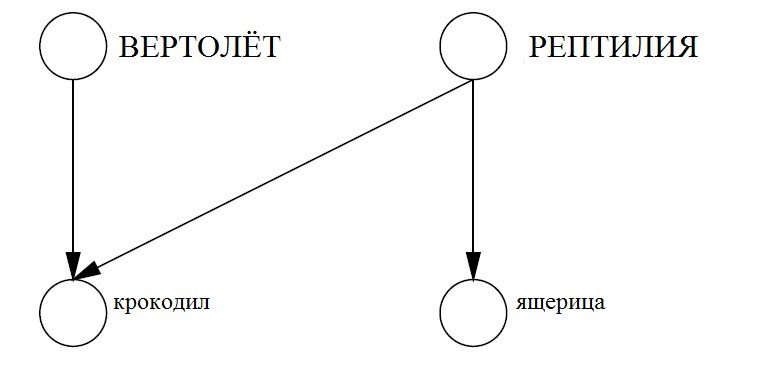
\includegraphics[keepaspectratio=true,width=0.9\columnwidth]{bayesian_network_crocodile.jpg}
    \caption{Байесовская сеть для многозначного существительного \textit{крокодил}}
    \label{ris1}
\end{figure}
\parindent=0,5cm

Глагол \textit{ползать} употребляется со словами \textit{крокодил} и \textit{ящерица}. Переменные ВЕРТОЛЕТ и РЕПТИЛИЯ соответствуют более общим абстрактным значениям, переменные \textit{крокодил} и \textit{ящерица} являются более узкими, конкретными значениями. Переменная РЕПТИЛИЯ может принимать одно из двух значений, соответствующих словам \textit{крокодил} и \textit{ящерица}, именно эту задачу определения значения и нужно решить.

\begin{table}[H]
\centering
\caption{Условные вероятности переменных \textit{крокодил} и \textit{ящерица} в зависимости от значений переменных ВЕРТОЛЕТ и РЕПТИЛИЯ, где (В, Р, к, я --- это аббревиатуры слов ВЕРТОЛЕТ, РЕПТИЛИЯ, \textit{крокодил} и \textit{ящерица})}
\begin{tabular}{|c|c|c|c|c|}
\hline
%" " & \multicolumn{4}{|c|}{ \textit{Р}(\textit{X = x}$\vert$\textit{Y_1 = y_1, Y_2 = y_2})} \\
" " & \multicolumn{4}{|c|}{ $Р(X=x|Y_1=y_1,Y_2=y_2)$ } \\
\hline
" " & В,Р & В,\textlnot Р & \textlnot В,Р & \textlnot В, \textlnot Р\\
\hline
к = \textit{true} & 0,99 & 0,99 & 0,99 & 0,01\\
к = \textit{false} & 0,01 & 0,01 & 0,01 & 0,99\\
\hline
я = \textit{true} & 0,99 & 0,99 & 0,01 & 0,01\\
я = \textit{false} & 0,01 & 0,01 & 0,99 & 0,99\\
\hline
\end{tabular}
\label{tbl1}
\end{table}

\parindent=0,5cm
При построении Табл.~\ref{tbl1} условных вероятностей (CPT), учтем следующие предположения:

\begin{itemize}
\item вероятность, что выбираем какой-либо из концептов (ВЕРТОЛЕТ и РЕПТИЛИЯ) очень мала, то есть \textit{P}(\textit{В=true}) = \textit{P}(\textit{Р=true}) = 0,01, следовательно, велика вероятность, что концепты не выбраны: \textit{P}(\textit{В=false}) = \textit{P}(\textit{Р= false}) = 0,99;
\item если какой-либо из концептов истинен (В, Р), то <<выпадает>> слово \textit{крокодил};
\item если концепт РЕПТИЛИЯ истинен, то растут шансы встретить слово \textit{ящерица};
\end{itemize}
\parindent=0,5cm

Из Табл.~\ref{tbl1} вероятности появления слов следует вывод, что использование разу двух значений слова \textit{крокодил (рептилия и вертолет МИ-24)} маловероятно. Вероятность использования значения РЕПТИЛИЯ намного больше чем значения ВЕРТОЛЕТ. Таким образом гипотеза <<вертолет>> <<отброшена>> (“explaining away”).
\parindent=0,5cm

\textbf{Байесовские сети для построения SP.} 
Иерархия существительных в WordNet представлена в виде ориентированного ацикличного графа. 
Синсет узла принимает значение <<истина>>, если глагол <<выбирает>> существительное из набора синонимов. 
Априорные вероятности задаются на основе двух предположений: во-первых, маловероятно, 
что глагол будет употребляться только со словами какого-то конкретного синсета, 
и во-вторых, если глагол действительно употребляется только со словами из данного синсета (например, синсет ЕДА), 
тогда должно быть правомерным употребление этого глагола с гипонимами этого синсета (например, ФРУКТ).
\parindent=0,5cm

Те же предположения (что для синсетов) верны и для употреблений слов с глаголами:
\begin{enumerate}
\item слово, вероятно, является аргументом глагола в том случае, если глагол употребляется с каким-либо из значений этого слова;
\item отсутствие связки глагол-синсет говорит о малой вероятности того, что слова этого синсета употребляются с глаголом.
\end{enumerate}
\parindent=0,5cm

Словам <<вероятно>> и <<маловероятно>> должны быть приписаны такие числа, сумма которых равна единице. 
\parindent=0,5cm

Находкой работы \cite{Ciaramita 2000} является разъяснение стратегии “explaining away”, то есть отбрасывание маловероятных значений слов при построении сочетаемостных ограничений. Такая стратегия является неотъемлемым свойством байесовских сетей и байесовского вывода, полезным свойством при разрешении лексической многозначности. 

\section{Заключение}

Разрешение лексической многозначности - это задача выбора между разными значениями слов и словосочетаний в словаре в зависимости от контекста. Задача разрешения лексической многозначности является открытой проблемой, то есть крайне интересной и привлекательной с научной точки зрения.

В статье представлен краткий обзор методов и алгоритмов разрешения лексической многозначности. Во-первых, методы, основанные на машинном обучении.  Во-вторых, методы, не использующие никаких размеченных корпусов для различения значений слов. В-третьих, методы, использующие внешние словарные источники информации (машиночитаемые словари, тезаурусы, онтологии).

Работа Старковой В.Г. поддержана грантом РГНФ (проект № 15-04-12029), работа Кириллова А.Н. и Чирковой Ю.В. поддержана грантом РГНФ (проект № 15-04-12006). Работа Крижановского А. А. выполнена при частичной финансовой поддержке Программы фундаментальных исследований Секции литературы и языка ОИФН РАН «Язык  и информационные технологии» 2015-2017 (проект "Корпус вепсского языка: разработка и формирование морфологической базы электронного ресурса").
 
\begin{thebibliography}{9}

\bibitem{Averin 2006}
\textit{Аверин А. Н.} Разработка сервиса поиска биграмм // Труды международной конференции «Корпусная лингвистика–2006. СПб., С.Петерб. ун-та., 2006.

\bibitem{epr:website}
\textit{Епрев А. С.} Применение контекстных векторов в классификации текстовых документов. 2010. http://jre.cplire.ru/iso/oct10/1/text.html.

\bibitem{Kim 1989}
\textit{Ким Дж. О., Мьюллер Ч. У., Клекка У. Р.} Факторный, дискриминантный и кластерный анализ. <<Финансы и статистика>>, Москва, Россия. 1989. Стр.172.

\bibitem{Lukash 2011}
\textit{Лукашевич Н. В.} Тезаурусы в задачах информационного поиска. Издательство МГУ, 2011. 495 с.

\bibitem{Trudakov 2010}
\textit{Турдаков Д. Ю.} Методы и программные средства разрешения лексической многозначности терминов на основе сетей документов: диссертация ... кандидата физико-математических наук: 05.13.11. --- Москва, 2010. --- 138 c.

\bibitem{Abney 1999}
\textit{Abney S. and Light M.} Hiding a semantic hierarchy in a markov model. In Proceedings of the Workshop on Unsupervised Learning in Natural Language Processing, ACL. 1999.

\bibitem{Azzini}
\textit{Azzini A., da Costa Pereira C., Dragoni M. and Tettamanzi A. G. B.} Evolving Neural Networks for Word Sense Disambiguation // 8-th International conference on hybrid intelligent systems. Spain. Barcelona. pp. 332–337. DOI: 10.1109/HIS.2008.88

\bibitem{Barzilay Elhadad 1997}
\textit{Barzilay R. and  Elhadad M. }Using lexical chains for text summarization. In Proceedings of the ACL Workshop on Intelligent Scalable Text Summarization (Madrid, Spain). 1997. pp. 10–17.

\bibitem{Berry 1993}
\textit{Berry M.,  Do T.,  O’Brien G.,  Krishna V. and Varadhan S. }SVDPACK (version 1.0) user’s guide. Technical Report CS-93-194, University of Tennessee at Knoxville, Computer Science Department, April 1993.

\bibitem{Bruce 1994}
\textit{Bruce R. and  Wiebe J. }Word-sense disambiguation using decomposable models. In Proceedings of the 32nd Annual Meeting of the Association for Computational Linguistics, 1994, pp. 139–146. DOI: 10.3115/981732.981752

\bibitem{Ciaramita 2000}
\textit{Ciaramita M. and  Johnson M. }Explaining away ambiguity: Learning verb selectional preference with Bayesian networks. 2000. 

\bibitem{COTTRELL 1983}
\textit{Cottrell G. W. and  Small S. L. }A connectionist  scheme for modelling word  sense  disambiguation -- Cognition and brain theory. 1983. № 6. pp. 89–120. 

\bibitem{COTTRELL 1989}
\textit{Cottrell G. W. }A connectionist approach to word sense disambiguation. Pitman, London, 1989.

\bibitem{Do Thuy Duong 2011}
\textit{Duong D. T. }Automated text summarization. Graduation Thesis. Hanoi University. 2011. 

\bibitem{Donald 1990}
\textit{Hindle D. }Noun classification from predicate-argument structures. In Proceedings of ACL-90, Pittsburg, Pennsylvania, June, 1990, pp. 268-275.

%\bibitem{Charles 1993}
%\textit{Ling Charles X.,  Marinov M. }Answering the connectionist challenge: A symbolic model of learning the past tenses of English verbs,  %Cognition, Elsevier, 1993.

%\bibitem{Dekang 1998}
%\textit{Lin D. }Automatic Retrieval and Clustering of Similar Words.Proceedings of the 17th international conference on Computational %linguistics-Volume 2. – Association for Computational Linguistics, Department of Computer Science University of Manitoba Winnipeg, Manitoba, %Canada, 1998, pp. 768-774. DOI: 10.3115/980432.980696

%\bibitem{Dekang 1993}
%\textit{Lin D. }Principle-based parsing without overgeneration. In Proceedings of ACL-93, Columbus, Ohio, 1993, pp. 112-120. DOI: %10.3115/981574.981590

%\bibitem{Dekang 1997}
%\textit{Lin D. }Using syntactic dependency as local context to resolve word sense ambiguity. In Proceedings of ACL/EACL-97, Madrid, Spain, %July, 1997, pp. 64-71. DOI: 10.3115/979617.979626

%\bibitem{Donald 1990}
%\textit{Hindle D. }Noun classification from predicate-argument structures. In Proceedings of ACL-90, Pittsburg, Pennsylvania, June, 1990, pp. %268-275.

%\bibitem{Do Thuy Duong 2011}
%\textit{Duong D. T. }Automated text summarization. Graduation Thesis. Hanoi University. 2011. 

\bibitem{Freund 1999}
\textit{Freund Y., Schapire R. E. }A Short Introduction to Boosting//AT\&T Labs Research, Shannon Laboratory. - 1999.

\bibitem{Freund 1996}
\textit{Freund Y.,  Schapire R. E. }Game theory, on-line prediction and boosting. In Proceedings of the Ninth Annual Conference on Computational Learning Theory,  1996. pp. 325-332.

\bibitem{Freund 1997}
\textit{Freund Y.,  Schapire R. E. }A decision-theoretic generalization of on-line learning and an application to boosting. Journal of Computer and System Sciences. 1997. pp. 119–139. DOI: 10.1006/jcss.1997.1504

\bibitem{Halliday Hasan 1976}
\textit{Halliday M. and  Hasan R. }Cohesion in English. London: Longman. 1976. 

\bibitem{Harris 1985}
\textit{Harris Z. }Distributional structure. In: Katz, J. J. (ed.) The Philosophy of Linguistics. New York: Oxford University Press. 1985. pp. 26–47

\bibitem{Hearst 1994}
\textit{Hearst M. }Multi-paragraph segmentation of expository text. In Proceedings of the 32th Annual Meeting of the Association for Computational Linguistics, 9–16. Las Cruces, New Mexico: Association for Computational Linguistics. 1994. DOI: 10.3115/981732.981734

\bibitem{Hinton 1986}
\textit{Hinton G. E.,  McClelland J. L.,  Rumelhart D. E.. }Distributed representations// In Parallel Processing: explorations in the microstructure of cognition. MIT Press, Cambridge, MA, 1986. pp. 5–44.

\bibitem{Hirst St-Onge 1998}
\textit{Hirst G. and  St-Onge D. }Lexical chains as representations of context for the detection and correction of malapropisms. WordNet: An electronic lexical database, 1998. pp. 305-332.

\bibitem{Hoey 1991}
\textit{Hoey M. }Patterns of Lexis in Text. Oxford: Oxford University Press. 1991. 

\bibitem{Jain 1988}
\textit{Jain A. and  Dubes R. }Algorithms for Clustering Data. Prentice-Hall, Inc., Upper Saddle River, NJ, 1988.

\bibitem{Jain 1999}
\textit{Jain A.,  Murthy M. and  Flynn P. }Data clustering: a review. ACM Computing Surveys, 31(3):264-323, September 1999. DOI: 10.1145/331499.331504

\bibitem{Leacock 1993}
\textit{Leacock C.,  Towell G. and  VoorheesE. }Corpus-based statistical sense resolution. In Proceedings of the ARPA Workshop on Human Language Technology, March. 1993, pp. 260–265.  

\bibitem{LESK 1986}
\textit{Lesk M. }Automatic sense disambiguation using machine readable dictionaries: How to tell a pine cone from an ice cream cone --  Proceedings  of  the 5th SIGDOC. New York. 1986. pp. 24–26. DOI: 10.1145/318723.318728

\bibitem{Dekang 1998}
\textit{Lin D. }Automatic Retrieval and Clustering of Similar Words.Proceedings of the 17th international conference on Computational linguistics-Volume 2. – Association for Computational Linguistics, Department of Computer Science University of Manitoba Winnipeg, Manitoba, Canada, 1998, pp. 768-774. DOI: 10.3115/980432.980696

\bibitem{Dekang 1993}
\textit{Lin D. }Principle-based parsing without overgeneration. In Proceedings of ACL-93, Columbus, Ohio, 1993, pp. 112-120. DOI: 10.3115/981574.981590

\bibitem{Dekang 1997}
\textit{Lin D. }Using syntactic dependency as local context to resolve word sense ambiguity. In Proceedings of ACL/EACL-97, Madrid, Spain, July, 1997, pp. 64-71. DOI: 10.3115/979617.979626


\bibitem{Lin 2001}
\textit{Lin D. and Pantel P. }Induction of semantic classes from natural language text. In Proceedings of SIGKDD-01. San Francisco, CA. 2001. pp. 317–322. DOI: 10.1145/502512.502558  

\bibitem{Charles 1993}
\textit{Ling Charles X.,  Marinov M. }Answering the connectionist challenge: A symbolic model of learning the past tenses of English verbs,  Cognition, Elsevier, 1993.


\bibitem{Manning 1999}
\textit{Manning C. D. and  Sch\"utze H. }Foundations of Statistical Natural Language Processing. MIT Press. 1999.

\bibitem{Merz 1998}
\textit{Merz C. J. and  Murphy P. M. }UCI repository of machine learning databases, 1998. www.ics.uci.edu/ mlearn/MLRepository.html.

\bibitem{Miller 1990}
\textit{Miller G. }Wordnet: An on-line lexical database. International Journal of Lexicography, 3(4). 1990.

\bibitem{Mooney 1996}
\textit{Mooney R. J. }Comparative Experiments on Disambiguating Word Senses:
An Illustration of the Role of Bias in Machine Learning, Department of Computer Sceinces, University of Texas, Austin, TX 78712-1188, 1996.

\bibitem{Mooney 1995}
\textit{Mooney R. J., Califf M. E. }Induction of First-Order Decision Lists: Results on Learning the Past Tense of English Verbs, Department of Computer Sceinces, University of Texas, Austin, TX 78712-1188, 1995.

\bibitem{Morris Hirst, 1991}
\textit{Morris J. and  Hirst G. }Lexical cohesion computed by thesaural relations as an indicator of the structure of text. Computational Linguistics 17(1):21–43. 1991. 

\bibitem{Navigli 2009}
\textit{Navigli R. }Word sense disambiguation: A survey. ACM Computing Surveys (CSUR) 41, no. 2 (2009): 10. DOI: 10.1145/1459352.1459355

\bibitem{Eugene 1975}
\textit{Nida Eugene A. }Componential Analysis of Meaning. The Hague, Mouton. 1975.


\bibitem{Pantel 2002}
\textit{Pantel P.,  Lin D. }Discovering Word Senses from Text. University of Alberta. Department of Computing Science Edmonton, Alberta T6H 2E1 Canada, 2002. DOI: 10.1145/775047.775138

\bibitem{Pedersen 2000}
\textit{Pedersen T. }A Simple Approach to Building Ensembles of Naive Bayesian Classi?ers for Word Sense Disambiguation// Department of Computer Science, University of Minnesota Duluth.–2000.

\bibitem{Pedersen 1997}
\textit{Pedersen T. and  Bruce R. }Distinguishing word senses in untagged text. Proc.EMNLP.Providence, RI, 1997.

\bibitem{Purandare 2004}
\textit{ Purandare A. and  Pedersen T. }Improving word sense discrimination with gloss augmented feature vectors // Workshop on Lexical Resources for the Web and Word Sense Disambiguation. – 2004. – pp. 123-130. 

\bibitem{Quinlan 1993}
\textit{Quinlan J. R. }C4.5: Programs for Machine Learning. Morgan Kaufmann, 1993. 

\bibitem{Resnik 1997}
\textit{Resnik P. }Selectional preference and sense disambiguation. In Proceedings of the ANLP-97 Workshop: Tagging Text with Lexical Semantics: Why, What, and How? 1997.

\bibitem{Savova 2005}
\textit{Savova G. }Resolving ambiguities in biomedical text with unsupervised clustering approaches. University of Minnesota Supercomputing Institute Research Report, 2005.

\bibitem{Schapire 1998}
\textit{Schapire R. E. and Singer Y. }Improved boosting a predictions. In Proceedings of the Eleventh Annual Confere Theory, 1998. pp. 80–91. 

\bibitem{Schapire 1997}
\textit{Schapire R. E. }Using output codes to boost multiclass learning problems. InMachin Learning: Proceedings of the Fourteenth International Conference, 1997. pp. 313–321. 

\bibitem{Schutze 1998}
\textit{Schutze H. }Automatic Word Sense Discrimination. Computational Linguistics, vol. 24, number 1., 1998.

\bibitem{SC:website}
\textit{SenseClusters. }  \newline http://senseclusters.sourceforge.net (дата обращения: ..........).

\bibitem{UMLS:website}
\textit{UMLS Terminology Services (UTS).} http://umlsks.nlm.nih.gov/kss/servlet/Turbine/\newline template (дата обращения: ..........)

\bibitem{VERONIS 1990}
\textit{Veronis J. and Ide N. }Word  sense  disambiguation  with  very  large neural  networks  extracted  from machine readable dictionaries – Proceedings of the 13th International Conference on Computational Linguistics. Helsinki. 1990. pp. 389–394. DOI: 10.3115/997939.998006

\bibitem{WALTZ 1985}
\textit{Waltz D. L. and  Pollack J. B. }Massively parallel parsing: a strongly interactive  model  of  natural  language interpretation – Cognitive science. 1985. № 9. pp. 51–74. DOI: 10.1207/s15516709cog0901\_4
                     
\bibitem{Weeber 2001}
\textit{Weeber M.,  Mork J.,  Aronson A. }Developing a test collection for biomedical word sense disambiguation. Proc. AMIA., 2001.

\bibitem{Zhao 2002}
\textit{Zhao Y. and  Karypis G. }Evaluation of hierarchical clustering algorithms for document datasets. In Proceedings of the 11th International Conference on Information and Knowledge Management, McLean, VA, 2002. pp. 515-524. DOI: 10.1145/584792.584877



\end{thebibliography}
\end{articletext}


\section{СВЕДЕНИЯ ОБ АВТОРE:}

\begin{aboutauthors}
\authorsname{Каушинис Татьяна Викторовна}
Студентка\\
Математический факультет\\ 
Петрозаводский государственный университет\\
пр-кт Ленина, 33, Петрозаводск, Республика Карелия\\
тел.: (8142) 711078\\
эл. почта: merilstreet@mail.ru

\columnbreak

\authorsname{Kaushinis, Tatiana}
Petrozavodsk State University\\
33, Lenin Str., 185910, Petrozavodsk, Republic of Karelia, Russia\\
tel.: (8142) 711078\\
e-mail: merilstreet@mail.ru
\end{aboutauthors}

\begin{aboutauthors}
\authorsname{Кириллов Александр Николаевич}
доктор физико-математических наук\\ 
доцент\\
Институт прикладных математических исследований Карельского научного центра РАН\\ 
ул. Пушкинская, 11, Петрозаводск, Республика Карелия, Россия, 185910\\
эл. почта: kirillov@krc.karelia.ru\\
тел.: (8142) 766312

\columnbreak

\authorsname{Kirillov, Alexander}
Institute of Applied Mathematical Research, Karelian Research Centre, Russian Academy of Sciences\\
11 Pushkinskaya St., 185910 Petrozavodsk, Karelia, Russia\\
e-mail: kirillov@krc.karelia.ru\\
tel.: (8142) 766312
\end{aboutauthors}

\begin{aboutauthors}
\authorsname{Коржицкий Никита Иванович}
Студент\\
Математический факультет\\ 
Петрозаводский государственный университет\\
пр-кт Ленина, 33, Петрозаводск, Республика Карелия\\
тел.: (8142) 711078\\
эл. почта: nikita@nikita.tv

\columnbreak

\authorsname{Korzhitsky, Nikita}
Petrozavodsk State University\\
33, Lenin Str., 185910, Petrozavodsk, Republic of Karelia, Russia\\
tel.: (8142) 711078\\
e-mail: nikita@nikita.tv 
\end{aboutauthors}

\begin{aboutauthors}
\authorsname{Крижановский Андрей Анатольевич}
кандитат технических наук\\ 
Институт прикладных математических исследований Карельского научного центра РАН\\ 
ул. Пушкинская, 11, Петрозаводск, Республика Карелия, Россия, 185910\\
эл. почта: andew.krizhanovsky@gmail.com\\
тел.: (8142) 766312

\columnbreak

\authorsname{Krizhanovsky, Andrew}
Institute of Applied Mathematical Research, Karelian Research Centre, Russian Academy of Sciences\\
11 Pushkinskaya St., 185910 Petrozavodsk, Karelia, Russia\\
e-mail: andew.krizhanovsky@gmail.com\\
tel.: (8142) 766312
\end{aboutauthors}

\begin{aboutauthors}
\authorsname{Пилинович Александр}
Студент\\
Математический факультет\\ 
Петрозаводский государственный университет\\
пр-кт Ленина, 33, Петрозаводск, Республика Карелия\\
тел.: (8142) 711078\\
эл. почта: alexander.pilinovich@yandex.ru

\columnbreak

\authorsname{Pilinovich, Aleksander}
Petrozavodsk State University\\
33, Lenin Str., 185910, Petrozavodsk, Republic of Karelia, Russia\\
tel.: (8142) 711078\\
e-mail: alexander.pilinovich@yandex.ru 
\end{aboutauthors}

\begin{aboutauthors}
\authorsname{Сихонина Ирина Александровна}
Студентка\\
Математический факультет\\ 
Петрозаводский государственный университет\\
пр-кт Ленина, 33, Петрозаводск, Республика Карелия\\
тел.: (8142) 711078\\
эл. почта: syawenka@mail.ru

\columnbreak

\authorsname{Sikhonina, Irina}
Petrozavodsk State University\\
33, Lenin Str., 185910, Petrozavodsk, Republic of Karelia, Russia\\
tel.: (8142) 711078\\
e-mail: syawenka@mail.ru 
\end{aboutauthors}

\begin{aboutauthors}
\authorsname{Спиркова Анна Михайловна}
Студентка\\
Математический факультет\\ 
Петрозаводский государственный университет\\
пр-кт Ленина, 33, Петрозаводск, Республика Карелия\\
тел.: (8142) 711078\\
эл. почта: annspirkova@gmail.com

\columnbreak

\authorsname{Spirkova, Anna}
Petrozavodsk State University\\
33, Lenin Str., 185910, Petrozavodsk, Republic of Karelia, Russia\\
tel.: (8142) 711078\\
e-mail: annspirkova@gmail.com
\end{aboutauthors}

\begin{aboutauthors}
\authorsname{Старкова Валентина Геннадьевна}
старший инженер-программист\\ 
Институт прикладных математических исследований КарНЦ РАН\\ 
ул. Пушкинская, 11, Петрозаводск, Республика Карелия, Россия, 185910\\
тел.: (8142) 766312\\
эл. почта: stark\_val@mail.ru

\columnbreak

\authorsname{Starkova, Valentina}
Institute of Applied Mathematical Research, Karelian Research Centre, Russian Academy of Sciences\\
11 Pushkinskaya St., 185910 Petrozavodsk, Karelia, Russia\\
tel.: (8142) 766312\\
e-mail: stark\_val@mail.ru 
\end{aboutauthors}

\begin{aboutauthors}
\authorsname{Степкина Татьяна Владимировна}
Студентка\\
Математический факультет\\ 
Петрозаводский государственный университет\\
пр-кт Ленина, 33, Петрозаводск, Республика Карелия\\
тел.: (8142) 711078\\
эл. почта: hogdp@mail.ru

\columnbreak

\authorsname{Stepkina, Tatiana}
Petrozavodsk State University\\
33, Lenin Str., 185910, Petrozavodsk, Republic of Karelia, Russia\\
tel.: (8142) 711078\\
e-mail: hogdp@mail.ru
\end{aboutauthors}

\begin{aboutauthors}
\authorsname{Ткач Станислав Сергеевич}
Студент\\
Математический факультет\\ 
Петрозаводский государственный университет\\
пр-кт Ленина, 33, Петрозаводск, Республика Карелия\\
тел.: (8142) 711078\\
эл. почта: tkachkras@gmail.com

\columnbreak

\authorsname{Tkach, Stanislav}
Petrozavodsk State University\\
33, Lenin Str., 185910, Petrozavodsk, Republic of Karelia, Russia\\
tel.: (8142) 711078\\
e-mail: tkachkras@gmail.com 
\end{aboutauthors}

\begin{aboutauthors}
\authorsname{Чиркова Юлия Васильевна}
кандидат физико-математических наук\\ 
Институт прикладных математических исследований КарНЦ РАН\\ 
ул. Пушкинская, 11, Петрозаводск, Республика Карелия, Россия, 185910\\
тел.: (8142) 766312
эл. почта: julia@krc.karelia.ru

\columnbreak

\authorsname{Chirkova, Julia}
Institute of Applied Mathematical Research, Karelian Research Centre, Russian Academy of Sciences\\
11 Pushkinskaya St., 185910 Petrozavodsk, Karelia, Russia\\
tel.: (8142) 766312
e-mail: julia@krc.karelia.ru
\end{aboutauthors}

\begin{aboutauthors}
\authorsname{Чухарев Алексей Леонидович}
старший инженер-программист\\ 
Институт прикладных математических исследований КарНЦ РАН\\ 
ул. Пушкинская, 11, Петрозаводск, Республика Карелия, Россия, 185910\\
тел.: (8142) 766312
эл. почта: chuharev@krc.karelia.ru

\columnbreak

\authorsname{Chuharev, Alexey}
Institute of Applied Mathematical Research, Karelian Research Centre, Russian Academy of Sciences\\
11 Pushkinskaya St., 185910 Petrozavodsk, Karelia, Russia\\
tel.: (8142) 766312
e-mail: chuharev@krc.karelia.ru
\end{aboutauthors}

\begin{aboutauthors}
\authorsname{Шорец Дарья Сергеевна}
Студентка\\ 
Математический факультет\\ 
Петрозаводский государственный университет\\
пр-кт Ленина, 33, Петрозаводск, Республика Карелия\\
тел: (8142) 711078\\
эл. почта: da\_sha1078@mail.ru

\columnbreak

\authorsname{Shorets, Daria}
Petrozavodsk State University\\
33, Lenin Str., 185910, Petrozavodsk, Republic of Karelia, Russia\\
tel.: (8142) 711078\\
e-mail: da\_sha1078@mail.ru
\end{aboutauthors}

\begin{aboutauthors}
\authorsname{Ярышкина Екатерина Александровна}
Студентка\\ 
Математический факультет\\ 
Петрозаводский государственный университет\\
пр-кт Ленина, 33, Петрозаводск, Республика Карелия\\
тел:(8142) 711078\\
эл. почта: kate.rysh@gmail.com

\columnbreak

\authorsname{Yaryshkina, Ekaterina}
Petrozavodsk State University\\
33, Lenin Str., 185910, Petrozavodsk, Republic of Karelia, Russia\\
tel.: (8142) 711078\\
e-mail: kate.rysh@gmail.com 
\end{aboutauthors}

\begin{aboutauthors}
\authorsname{Янкевич Дарья Юрьевна}
Студентка\\ 
Математический факультет\\ 
Петрозаводский государственный университет\\
пр-кт Ленина, 33, Петрозаводск, Республика Карелия\\
тел: (8142) 711078\\
эл. почта: dyankevic@gmail.com

\columnbreak

\authorsname{Yankevich, Daria}
Petrozavodsk State University\\
33, Lenin Str., 185910, Petrozavodsk, Republic of Karelia, Russia\\
tel.: (8142) 711078\\
e-mail: dyankevic@gmail.com
\end{aboutauthors}


\end{document}
